 \documentclass{article}

% if you need to pass options to natbib, use, e.g.:
% \PassOptionsToPackage{numbers, compress}{natbib}
% before loading nips_2016
%
% to avoid loading the natbib package, add option nonatbib:
% \usepackage[nonatbib]{nips_2016}

\PassOptionsToPackage{numbers,sort&compress}{natbib}
\usepackage[final]{nips_2016} % produce camera-ready copy

\usepackage[utf8]{inputenc} % allow utf-8 input
\usepackage[T1]{fontenc}    % use 8-bit T1 fonts
\usepackage{hyperref}       % hyperlinks
\usepackage{url}            % simple URL typesetting
\usepackage{booktabs}       % professional-quality tables
\usepackage{amsfonts}       % blackboard math symbols
\usepackage{nicefrac}       % compact symbols for 1/2, etc.
\usepackage{microtype}      % microtypography
\usepackage{graphicx}
\usepackage{color,soul}
\usepackage{bm}
\usepackage[table]{xcolor}
\usepackage{titlesec}
\usepackage{listings}
\usepackage{float}

\usepackage[skip=0.333\baselineskip]{caption}
\usepackage{subcaption}

\definecolor{codegreen}{rgb}{0,0.6,0}
\definecolor{codegray}{rgb}{0.5,0.5,0.5}
\definecolor{codepurple}{rgb}{0.58,0,0.82}
\definecolor{backcolour}{rgb}{0.95,0.95,0.92}

\lstdefinestyle{mystyle}{
    backgroundcolor=\color{backcolour},   
    commentstyle=\color{codegreen},
    keywordstyle=\color{magenta},
    numberstyle=\tiny\color{codegray},
    stringstyle=\color{codepurple},
    basicstyle=\ttfamily\footnotesize,
    breakatwhitespace=false,         
    breaklines=true,                 
    captionpos=b,                    
    keepspaces=true,                 
    numbers=left,                    
    numbersep=5pt,                  
    showspaces=false,                
    showstringspaces=false,
    showtabs=false,                  
    tabsize=2
}

\lstset{style=mystyle}

\title{Machine Learning for Species Analysis}

% The \author macro works with any number of authors. There are two
% commands used to separate the names and addresses of multiple
% authors: \And and \AND.
%
% Using \And between authors leaves it to LaTeX to determine where to
% break the lines. Using \AND forces a line break at that point. So,
% if LaTeX puts 3 of 4 authors names on the first line, and the last
% on the second line, try using \AND instead of \And before the third
% author name.

\author{
  Student number\\ s1910360
  %% examples of more authors
  \And
  Student number\\ s2572047
 \And
  Student number\\ s1922260
}

\titlespacing{\section}{1pt}{\parskip}{-\parskip}
\titlespacing{\subsection}{1pt}{\parskip}{-\parskip}
\titlespacing{\subsubsection}{1pt}{\parskip}{-\parskip}

\begin{document}

\maketitle

\begin{abstract}
 This report tackles the problem of species identification using location data, and a resultant analysis of the effect of climate change on specific species. We explore different types of population distribution and use these findings to accurately train and test several machine learning algorithms (\textbf{Logistic Regression}, \textbf{K-Nearest Neighbours}, \textbf{Random Forest} and \textbf{Feed-Forward Neural Networks}). We then compare models using AUC-ROC, AUC-PR, F2 scores, and Cohen's kappa, and further investigate implementing new bio-climatic variables to predict species affected by climate change and analyze the resultant F2 metric.
\end{abstract}

% \section*{Current progress}
To begin, we explored the training data provided. We looked at the number of data points, the number of
species, the number of observations for each species, and other statistical methods on the training data. Following we started with an exploratory analysis of the data, mainly focused on the distributions of observations for a few given species, calculating the largest and smallest span out of all species. We were also interested in the most commonly observed species and so we analysed all the species with the maximum number of observations and found in which continent these were most commonly observed. Next, we focused on a few different machine learning models and their application to
this data-set, with the goal of predicting the most likely species present at a given coordinate. The
models we’ve used so far are Gaussian classification, k-nearest neighbours classification, decision
trees, and neural networks. We have also started evaluating the accuracy of our models, understanding and manipulating the test data provided was a big part in doing this.


% \section*{Future plans}
Our first goal moving forward is to determine which of the four models we’ve used so far is the ’best’. For this, we will evaluate each model using some accuracy measure and compare the scores. We are looking at the F1 score at the moment. Once the optimal model has been determined, our next task is to determine which species are most affected by climate change, by combining our model predictions with climate data from WorldClim. Current idea is to find areas with biggest temperature change and determine most common species in those areas through our models.
\setlength{\textfloatsep}{2pt}

\section{Introduction}
A key problem in ecology is understanding the many ecosystems of the world and how they respond to climate change, conservation efforts, and habitat destruction. Central to this work is the monitoring of species present in a fixed area and collection of data from a variety of sources. Ecologists can then perform species distribution modelling (SDM) using this data and determine the species present in an ecosystem, their respective populations, and how these populations change over time. However, the processing and analysis of data can take years due to the large number of samples taken. Machine learning offers a promising method to speed up SDM.
%, allowing for larger studies across longer timescales. 
In this report, we use various machine learning models to analyse data from iNaturalist (\url{www.inaturalist.org}), a "crowd-sourced species identification system". We evaluate our machine learning methods to determine which has the best classification accuracy for this data-set, then attempt to improve the model capabilities by training on eight new bio-climatic variables from WorldClim \cite{worldclim}, visually explored in Appendix \ref{appendix:bio}. We use the most improved model in conjunction with projected temperature data from the Met Office Hadley Centre HadGEM3-GC31-LL model \cite{met} to subsequently determine which species are most affected by climate change, which could then be used to focus conservation efforts. 

\section{Background}

Machine learning methods have been used extensively in the context of SDM; see \cite{vincenzi2011application}, \cite{jin2012predicting}, \cite{jackson2015citizen}, \cite{aertsen2010comparison} for examples. Beery et. al. \cite{beery2021species} provide a comprehensive review of SDM aimed at computer scientists, highlighting the common methods, terminology, and challenges associated with this area.
A common practice in previous work is to combine geospatial data for a particular species with bioclimatic variables (e.g. temperature, precipitation) and topographical attributes (e.g. elevation, slope, flow water direction). Lorena et. al. \cite{lorena2011comparing} compare the use of nine different machine learning models in predicting the distribution of thirty five Latin American plant species. Geospatial data for each species was combined with nine environmental layers, comprising of four climatic variables and five topographical attributes. Lee et. al. \cite{lee2022spatial} used a similar approach to model the potential distribution of invasive ant species under climate change. This approach seems viable for our purposes.
%The authors suggest using an ensemble method to compensate for discrepancies between models, however Hao et. al. \cite{hao2020testing} found only a slight increase in performance using an ensemble model over an individual model using a data-set of eucalyptus tree species.

\section{Exploratory data analysis} \label{sec:explore}
% \hl{Dj: [Generic explanation of the structure of data, i.e. we received data split already; how many data points, how many species. Did each species have equal data points?(No), should address these q's.]}

% \hl{Dj: I think that we will need to be quite particular about what we place in exploratory data analysis -> should be relevant to our tasks.}

% \hl{Dj: whats written below is very rough and will need to be reworded etc..}
A brief overview of the available data structure is included in appendix \ref{appendix:datastruct}. Notably, the mean number of locations attributed to each species is much higher in the test data-set vs. the train data-set. The training data, sourced from citizen scientists, is noisy due to non-regularized collection methods, and important information relevant to  conservation efforts such as the observation date of the species is not provided. 
Additionally, the format of the two data-sets is different. The train data-set provides locations and a singular associated species, whereas the test data-set provides locations and a corresponding list of multiple species. It is important to note the difficulty that this may present in creating models that can accurately predict multiple species per location\footnote{This is because the training data-set provides us with data suited to a singular label classification problem, whereas the test data-set is suited toward a multi-label classification problem.}. The distribution of these two data-sets is best visualized through the plots given in Figure \ref{fig:dist_data}.

\begin{figure}[hbt!]
\centering

\begin{subfigure}{.32\linewidth}
\vspace*{-1ex}  
\begin{center}
\textbf{Train data-set}
\end{center}
\vspace*{-1ex}
  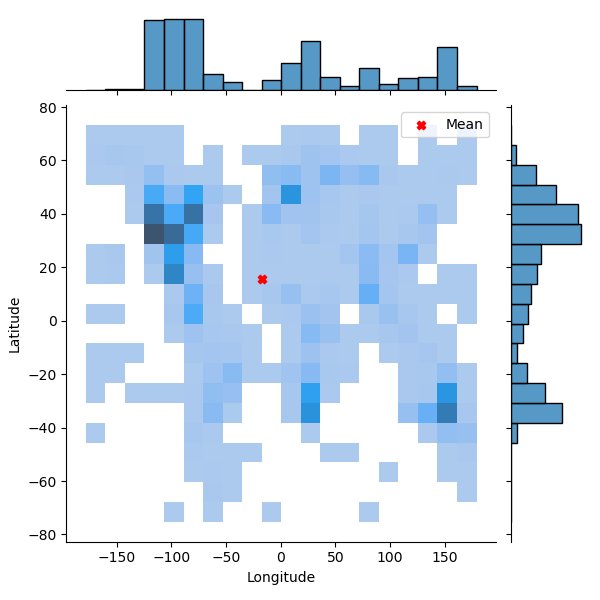
\includegraphics[width=\linewidth]{Images/hist_train.png}
\end{subfigure} % <-- "\hfill"
\begin{subfigure}{.32\linewidth}
\vspace*{-1ex}  
\begin{center}
\textbf{Test data-set}
\end{center}
\vspace*{-1ex}
  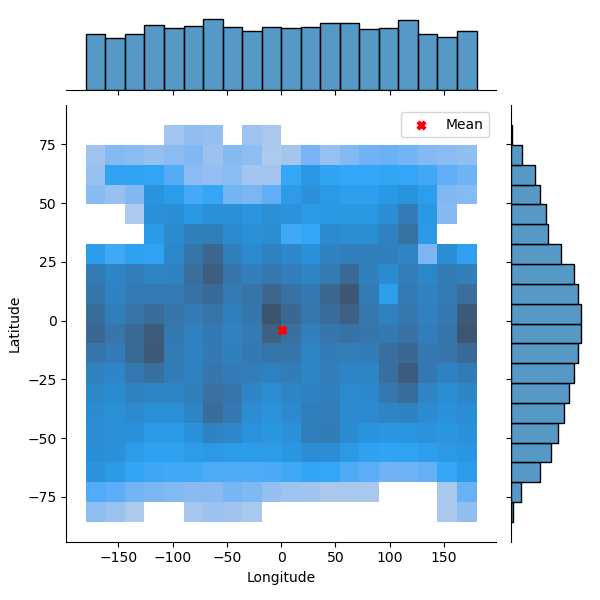
\includegraphics[width=\linewidth]{Images/hist_test.png}
\end{subfigure}
\begin{subfigure}{.32\linewidth}
\vspace*{-1ex}  
\begin{center}
\textbf{Avg. species observations per continent (train data-set)}
\end{center}
\vspace*{-1ex}
  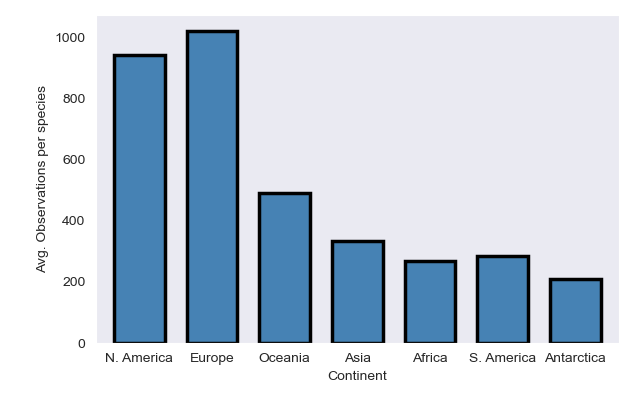
\includegraphics[width=\linewidth]{Images/obsve.png}
\end{subfigure}

\caption{Distribution of data from the train (left) and test (middle) data-sets at locations where there are species observation $\geq$ 1, note the offset mean location in the train data-set, and the centralized mean location in the test data-set. (Right) is a comparison of the number of observations per species in the train data-set for each continent.}
\label{fig:dist_data}
\end{figure}

Data from the training data-set is not evenly spread, with larger amounts of data associated with the longitude and latitude ranges (-120, -90) and (20, 50) for example, roughly corresponding to North America. This can be attributed to the fact that there may be more iNaturalist users in this region.
An analysis on the number of observations per species for each continent is subsequently carried out to further show this data imbalance.
A random sample of twenty locations (converted to a continent name) was taken for every species, and the most common continent among those twenty was taken to be the species continent. As shown in Figure \ref{fig:dist_data}, Europe has the highest number of observations (data-points) per species. This shows a clear bias in the data; species from Europe and North America have, on average, a larger number of observations. A more comprehensive table of this data is included in Appendix \ref{appendix:table1}. The test data-set on the other hand, considers a (roughly) even spread of location data points. Additionally, the species in the data-set have widely varying population distributions. 
Figure \ref{fig:dist} shows the extremes in species distribution span and density in the test data-set.
%Figure \ref{fig:dist} shows an analysis of the population distribution span and density of data in the train data-set, i.e. a comparison of the largest found distances and densities between data points of a species.

\begin{figure}[hbt!]
\centering

\begin{subfigure}{.45\linewidth}
\vspace*{-1ex}  
\begin{center}
\textbf{Species distribution span}
\end{center}
\vspace*{-1ex}
  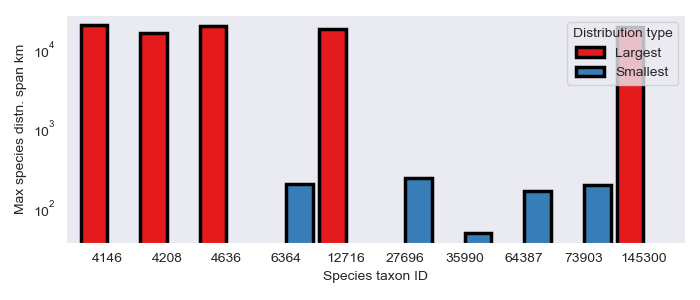
\includegraphics[width=\linewidth]{Images/large_small.png}
\end{subfigure}
\begin{subfigure}{.45\linewidth}
\vspace*{-1ex}  
\begin{center}
\textbf{Species distribution density}
\end{center}
\vspace*{-1ex}
  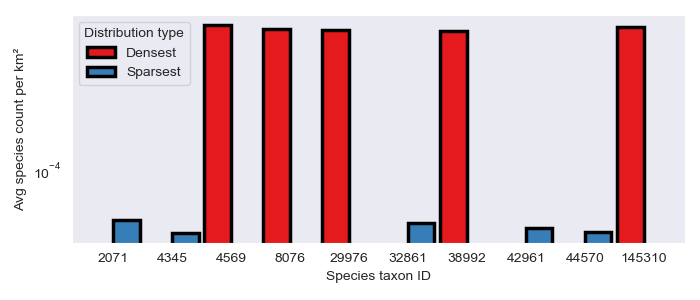
\includegraphics[width=\linewidth]{Images/dense_sparse.png}
\end{subfigure} % <-- "\hfill"

\caption{(Left) The variation on population distribution of 10 different species (top 5 largest vs top 5 smallest). (Right) The variation on population density of 10 different species (top 5 densest vs top 5 sparsest), note the logarithmic scaling of both plots.}
\label{fig:dist}
\end{figure}

Notably, population spans vary widely. An initial hypothesis is that this will affect a machine learning model's ability to correctly predict species distributions\footnote{Largely spread populations may provide less generalization for the ML models to learn about species population.}, and so this is something that we would like to investigate. 
Not only do the species population distributions span different distances, but they also have a wide range of densities. Some species have a much larger count in the train data-set attributed to a smaller area, whereas other species have small counts over larger areas.
A second hypothesis to consider is our machine learning methods' capability to predict sparse and dense population distributions\footnote{Sparsely spread populations provide less correlation for the ML models to learn, whereas dense populations have fewer outliers.}.

%Another way we analysed the data was by looking at the most commonly observed species. There are 64 species in the data-set with \hl{greater than?} 2000 observations (the maximum number). Out of these species, a random sample of 10 locations was taken to compute the most common continent in which these species are located. While 10 points aren’t much, calculating the continent of each coordinate requires a lot of computational power, and each species is “expected” to be mostly in the same continent. We found that most species with max observations were observed in North America with 42 and Europe with 12 while Oceania had 4, Africa and South America 2, and Asia 1. This clearly shows a big bias in where the data was collected. 

%Another way we analysed the data was by searching for the most and least commonly observed species. As shown in \ref{tab:my_continent} there are 72 species with more than 1500 locations. For all species, a random sample of 20 locations was taken to compute the most common continent in which these species were located. North America had the most species overall with 134, Africa was second with 122 and Europe was last with 34 (excepting Antarctica). Yet, for the most common species, Europe comes second to North America with 12 species while Africa only has 2. This shows a very clear bias in the data, while Africa has much more diversity, Europe has many more observations per species.

% \hl{can this paragraph be moved to where I highlighted ----}

% Finally, we analysed the data by searching for the most common continent for each species. A random sample of 20 locations (converted to a continent name) was taken for every species, the most common continent among those 20 was taken to be the species continent. As shown in appendix \ref{appendix:table1}, North America has the most number of species with 134, closely followed by Africa with 122, while Europe has the least with 34 (excepting Antarctica). However, the number of observations in Europe per species nearly quadruples those in Africa. This shows a clear bias in the data; species from Europe and North America have, on average, a lot more observations.% This reinforces the need to balance the data before training our models to prevent the model from being disproportionately influenced by labels from Europe and North America with an abundance of data. %This is consistent with what you would expect from "citizen scientists" as most of the iNaturalist community resides in these continents. 

%\hl{Would be interesting to check later on if we get a better accuracy for North America and Europe compared to the other continents? Is this possible computationally? Would possibly have to check the continent of every location – not realistic computationally. In any case this shows the importance of “data balancing” in some way. We will probably need to create weights for each specie.}


% Don't think we'll need to do the density one
% Additionally, further analysis of the distribution of species was done to analyze the density of populations

% \begin{figure}[h]
% \centering
% \includegraphics[width = \textwidth]{Images/Dense_spread.png}
% \caption{Largest found density of species (Hyla Chinensis) versus smallest (Larus occidentalis).}
% \end{figure}

\section{Data preparation}

%\hl{Explain efforts to balance data, creates weights for each species that can then be used in training the models.}

%\hl{Only consider test data at which species are present}

Through the exploratory analysis, it was evident that a significant imbalance existed within the data-set that needed to be considered before model training could begin. Imbalances in class distributions introduce bias during the training of the models, leading to a loss of performance. To avoid this, individual species weights were introduced via the equation\footnote{Note; this is the built-in weight equation from sk-learn.} 
\begin{lstlisting}[language=Python] 
species_weight = len(train_locs)/(species_count * no.species) 
\end{lstlisting}
These weights ensure that the models place more emphasis on species that may be underrepresented in the training data-set \cite{hashemi2018weighted}. This method then allowed for the whole data-set to be used in training the algorithms, unlike other methods such as sub-sampling which would sacrifice information about the data-set. Due to our data having only two features, latitude and longitude, dimensionality reduction is unneeded, as our data is already in a low-dimensional space (2D).
%a decision was made to bring labels with locations exceeding the mean down to this average level. The selection method involved randomly sub-sampling  544 data points. This process aimed to create a more equitable distribution of samples across all classes, creating an improved model for generalization. This model was chosen for its simplicity, allowing consistency across all models and easier interpretability, as well as for its positive results [\hl{This is what is harder to justify... I got better results using this balance method but they were "anecdotical", could we justify this another way?}].  By limiting the number of observations for certain species, the models are encouraged to learn more about the entire data-set, rather than being swayed by the prevalence of certain classes.




\section{A Species Distribution analysis using different Machine Learning methods}

The central goal of this task is to predict the different species found at a given set of specified coordinates (latitude, longitude) using a variety of machine learning methods. In our investigation, we analyze the multi-label, classification capabilities of 1.\ \textbf{Logistic Regression}, 2.\ \textbf{Random Forest}, 3.\ \textbf{K-Nearest Neighbour} \& 4.\ \textbf{Feed Forward Neural Network} models. With these four implemented methods we perform subsequent analysis to evaluate and compare the accuracy of each model. Having done so, we aim to answer questions such as the prevalence of specific species in given regions.

\textbf{Logistic Regression} is a simple but powerful linear model for classification which uses a logistic function to model the probability of a binary outcome. This was implemented using the built-in LogisticRegression implementation in scikit-learn. As we wish to study the per-class probabilities at each location, we use the multinomial method, which seeks to minimise the cross-entropy loss during training, rather than a one-versus-rest scheme. The softmax function is then used to calculate the per-class probabilities. The main disadvantage of logistic regression in this context is that the data is unlikely to be linearly separable; for example, if a particular species is distributed across two different continents. Despite this, the ease of implementation for logistic regression makes it an appealing model to study.
\textbf{Random Forests} are a suitable choice for our data-set due to their inherent ability to handle complex data and capture non-linear patterns \cite{breiman2001random}. The ensemble nature of Random Forests is useful to avoid over-fitting and allow for better generalization. Implementation-wise, the model was realized using the scikit-learn library, the number of estimators was set at 100 and the maximum depth was optimized by calculating the F1 scores for different depth values (see Appendix \ref{appendix:RFF1}). At \textit{max\_depth=10}, the performance of the model plateaus and so it was chosen to avoid over-fitting.
\textbf{K-Nearest Neighbours (KNN)} calculates the k-nearest neighbours to a data-point based on some chosen distance metric, then assigns a class based on whichever class makes up the majority of these neighbours. Using sci-kit learn's implementation, we chose $k = 75$ as the number of neighbours, determined by calculating the mean F1 score across all species for different values of $k$ (see Appendix \ref{appendix:KNNF1}). In addition, we use the standard Euclidean metric to determine the distance between points and neighbours. The per-class probabilities for a particular location are calculated as the number of neighbours belonging to each class divided by the total number of neighbours. %We expect KNN to work well for localised species distributions.%
\textbf{Feed-Forward Neural Networks (FFNN's)} are able to implicitly detect non-linear relationships through the use of a connected layer architecture. They are therefore a potentially suitable model to use to train population distributions. They were implemented using PyTorch. A visual of the implementation is provided in Appendix \ref{appendix:ffnn}.
Specifically, the model takes in longitude and latitude as features and passes them through a set of hidden layers using an activation function. The activation function used between hidden layers is a Rectified Linear unit (ReLu), and the output used a sigmoid activation to scale outputs between 1 \& 0 for a k-hot vector, i.e.\ species present or not.
Binary cross entropy was used to evaluate the loss of the model as it is best suited for a multi-label classification, and an Adam optimizer was implemented with a learning rate of 0.001 to best adjust the weights accordingly without over-fitting.


\subsection{Methods \& evaluation}

%In order to sufficiently evaluate the capabilities and subsequent drawbacks of the algorithms that we've explored, we've considered multiple AUC-ROC \& AUC-PR scores of the models and how they vary with different types of population distributions. Importantly, this unveils how models do with species with highly localised populations, widely distributed populations,  dense populations and sparse populations, all of which were initially explored in the data exploration, section \ref{sec:explore}.

%To comprehensively assess model performance, we employed several metrics, including AUC-ROC \& AUC-PR scores. To apply these we had to turn our problem into a binary classification one, hence we implemented a one-vs-rest approach whereas the confusion matrix values were found comparing the presence versus the absence of each species in the test data and the predictions. This allowed for a nuanced examination of the model's capability for individual labels. To generalize this, we found the average for 4 distinct groups as explored in section \ref{sec:explore} - the top 5 most dense, top 5 most sparse, top 5 smallest span and top 5 largest span, as well as the average over all species. An advantage of using AUC-ROC and AUC-PR is that it allows for easier comparison between models as it does not depend on the decision threshold which might be different for different models. They are also appropiate for problems with big class imbalances, which is our case given that the absence of a species class always dominates.

To comprehensively assess model performance, we utilized several metrics, including AUC-ROC \& AUC-PR scores. 
%To apply these, we  transformed our problem into a binary classification task using a one-vs-rest approach. This involved comparing the presence versus absence of each species in the test data and the corresponding model predictions. Allowing for a nuanced examination of the model's capability for individual labels.
To generalize our assessment, we calculated averages for four distinct groups as detailed in Section \ref{sec:explore}: the top 5 most dense, most sparse, smallest span, and largest span, along with an average across all 500 species. The advantage of employing AUC-ROC and AUC-PR is that they allow for easier comparison between models as they don't depend on the different decision thresholds. Considering the inherent class imbalances in our data-set, where the absence of a species class always dominates, precision and recall emerge as important metrics to evaluate \cite{saito2015precision}.

It is important to note that, given the nature of our project, our primary concern centers around positive class predictions. Consequently, AUC-PR scores assume greater relevance in our model assessment than AUC-ROC scores. Within the positive class, the emphasis is placed on minimizing false negatives for accurate species identification. To address this, we opted to evaluate F2 scores, providing a balanced measure of accuracy that prioritizes recall over precision.\footnote{F2 comes from the generalized F-Beta measure, $F(\beta)=(1+\beta)*Pr*Re/(\beta^2*Pr+Re)$; an increase in $\beta$ emphasizes the importance of Recall.}\cite{sasaki2007truth} We also evaluated Cohen’s Kappa (CK) to check whether agreement between predictions and reality is achieved by chance.\cite{warrens2015five}


\begin{figure}[hbt!] 
\centering


\begin{subfigure}{.45\linewidth}
\vspace*{-1ex}  
\begin{center}
\textbf{AUC-ROC}
\end{center}
\vspace*{-1ex}
  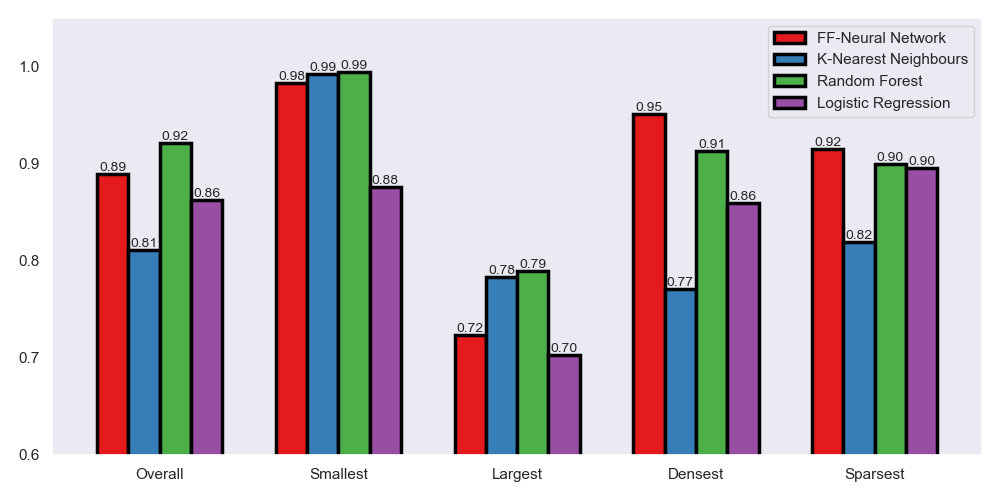
\includegraphics[width=\linewidth]{Images/AUC_ROC.png}
\end{subfigure}
  \hspace*{-1em}
\begin{subfigure}{.45\linewidth}
\vspace*{-1ex}  
\begin{center}
\textbf{Cohen kappa (CK)}
\end{center}
\vspace*{-1ex}
  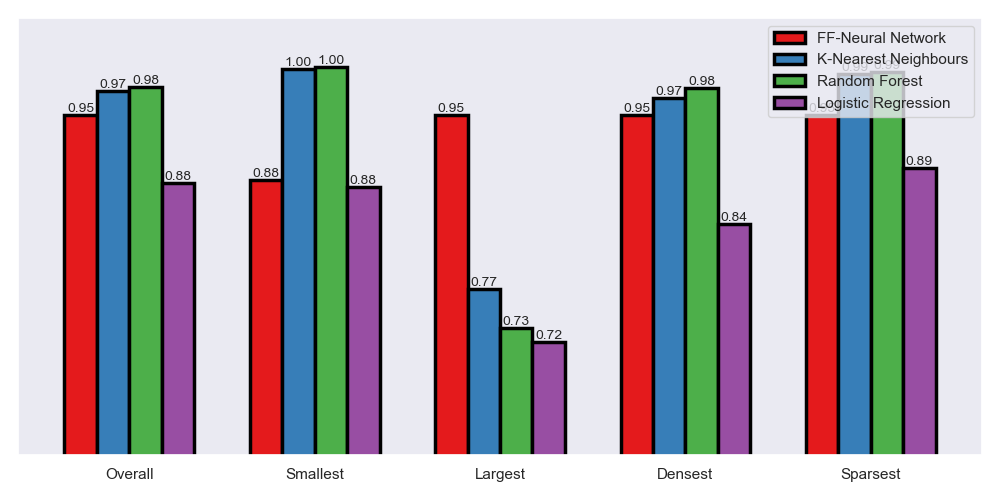
\includegraphics[width=\linewidth]{Images/Cohen_Kappa.png}
\end{subfigure}

\begin{subfigure}{.45\linewidth}
\vspace*{1ex}  
\begin{center}
\textbf{AUC-PR}
\end{center}
\vspace*{-1ex}
  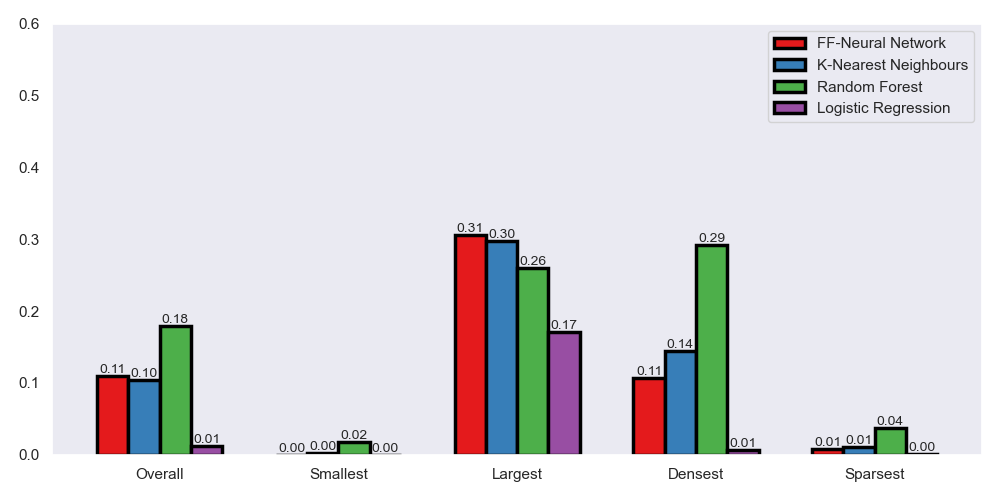
\includegraphics[width=\linewidth]{Images/AUC_PR.png} % f-measure
\end{subfigure}
  \hspace*{-1em}
\begin{subfigure}{.45\linewidth}
\vspace*{1ex}  
\begin{center}
\textbf{F2-measure}
\end{center}
\vspace*{-1ex}
  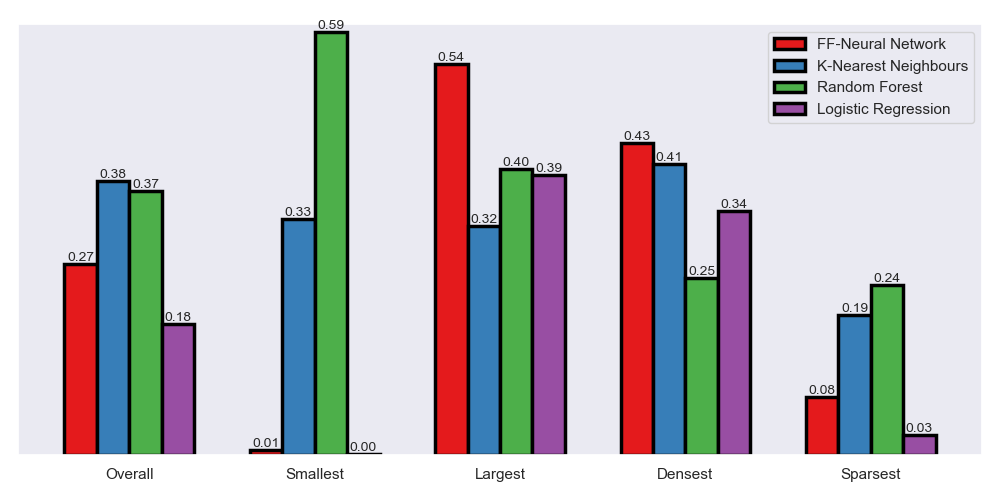
\includegraphics[width=\linewidth]{Images/F2 totals.png} % cohens kappa
\end{subfigure}


\caption{Model performance according to different population distribution types. For each population distribution type the top-5 were evaluated. Note the y axis range for AUC-ROC and Cohen's Kappa (0.6 - 1.0) as opposed to the range for AUC-PR and F-measure  (0.0 - 0.6).}
\label{fig:analysis}
\end{figure}

\subsection{Analysis \& results}

%From figure \ref{fig:analysis}, we see that models tend to achieve better AUC-ROC values with data that has a smaller distribution compared to larger distributions. The opposite is shown with the AUC-PR scores. This is because of the inherent imbalance in the test data; the smallest distributions were attributed to species in the data-set which had very low counts, for example, \emph{Gallotia Stehlini} had only 2 data-points. This skews the Precision and Recall to 0, as well as the False Positive Rate (increasing the ROC score). A variation is not observed between densest and sparsest for the ROC curves, but the densest distribution outperforms the PR score of the sparsest distribution. \hl{This is expected as dense distributions are easier to model/predict?}
From Figure \ref{fig:analysis}, we see that models tend to achieve better AUC-ROC values with data that has a smaller distribution compared to larger distributions. However, the opposite is found with the AUC-PR scores. This is because of the inherent imbalance in the test data; the smallest distributions were attributed to species in the data-set which had very low counts, for example, \emph{Gallotia Stehlini} (35990) had only 2 data-points. This skews the Precision and Recall to 0, as well as the False Positive Rate (increasing the ROC score). A variation is not observed between densest and sparsest for the ROC curves, but the densest distribution outperforms the PR score of the sparsest distribution. This result is expected as denser distributions are generally easier to model due to the data being highly correlated, kin to having fewer `outliers' \cite{ackerman2020detection}. The values for CK are all high, confirming the reliability of our models. The F2-score shows variability in performance between models and between the different distribution types, for example RF and KNN perform consistently well across all types yet FFNN and LR perform comparatively worse on the smallest and sparsest distributions. A visual exploration of results provides a more intuitive evaluation of our models' capabilities to predict species distributions (Figure \ref{fig:map}).

\vspace{-2ex}
\begin{figure}[hbt!]

\centering
\vspace*{-1ex}  
\begin{center}
\textbf{True distribution (test data-set)}
\end{center}
\vspace*{-1ex}
\begin{subfigure}{.3\linewidth}
  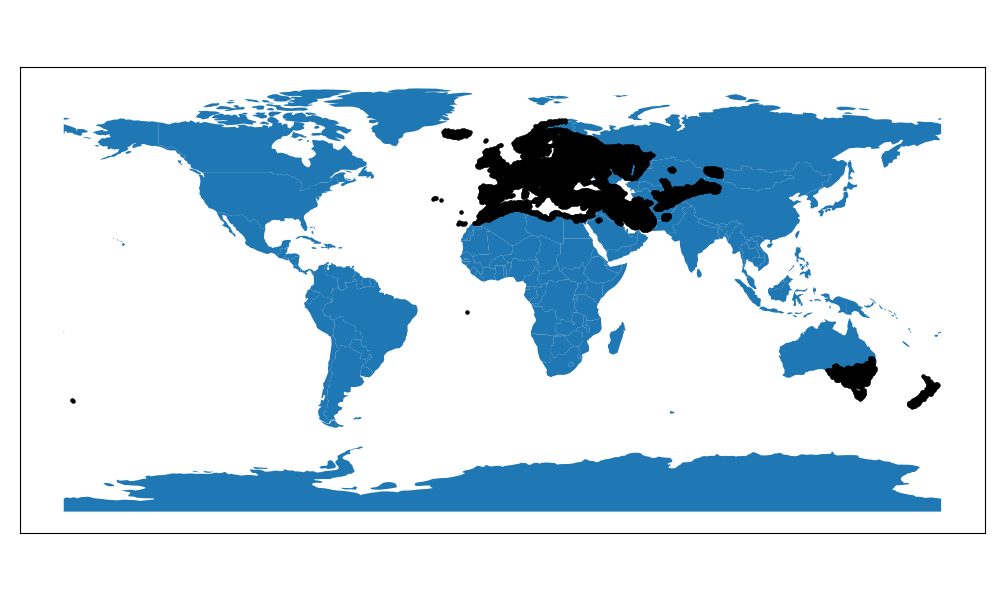
\includegraphics[width=\linewidth]{Images/turdus_true.png}
\end{subfigure} 
\vspace{-3ex}

\begin{subfigure}{.23\linewidth}
  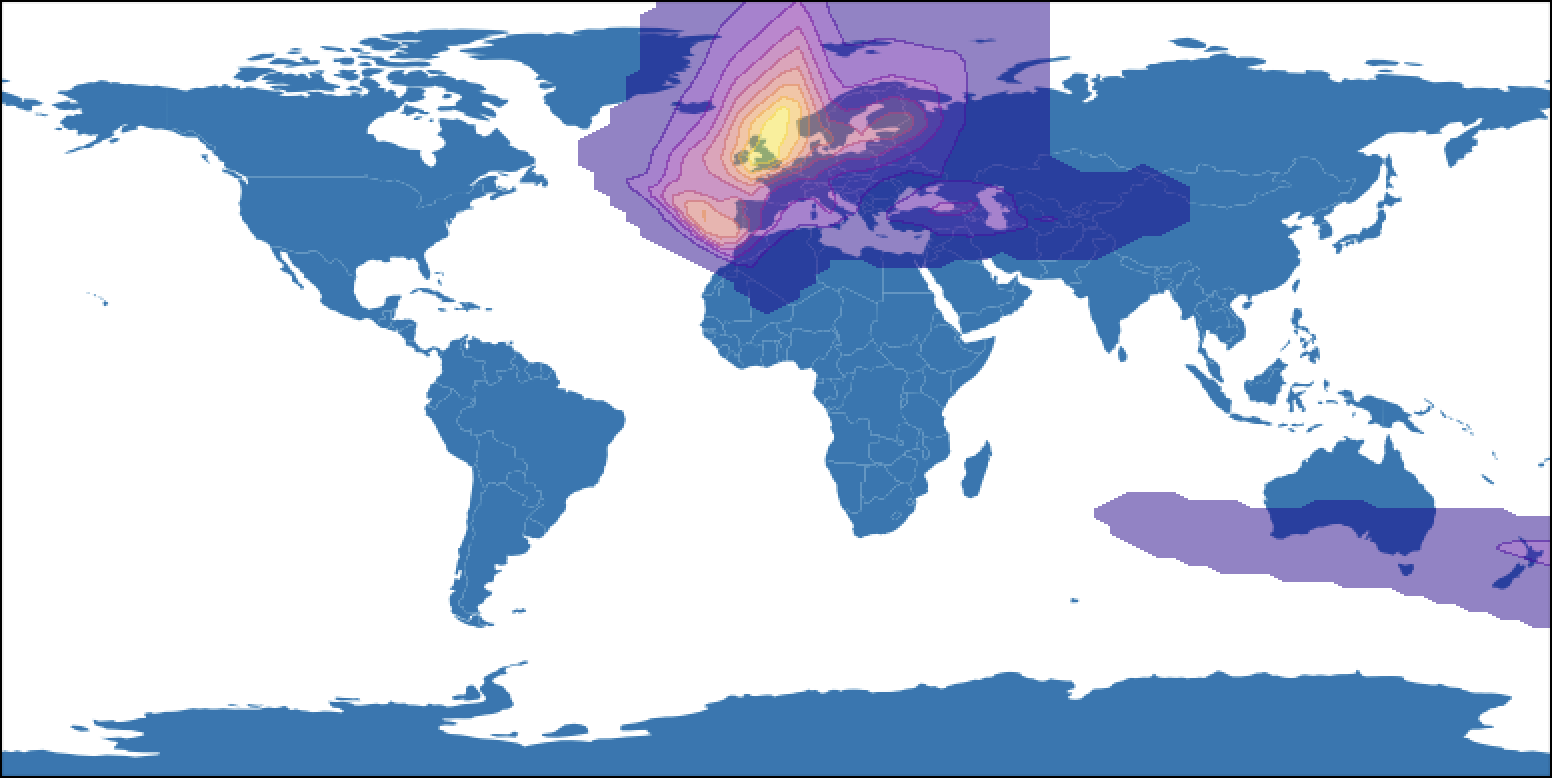
\includegraphics[width=\linewidth]{Images/Screenshot 2023-11-15 at 15.16.04.png}
\vspace*{-3ex}  
\begin{center}
\textbf{Feed-Forward NN}
\end{center}
\end{subfigure}
\begin{subfigure}{.23\linewidth}
  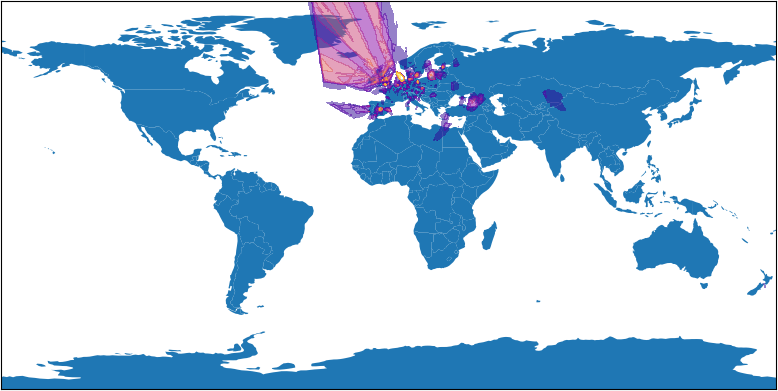
\includegraphics[width=\linewidth]{Images/knn_prediction.png}
\vspace*{-3ex}  
\begin{center}
\textbf{K-Nearest Neighbour}
\end{center}
\end{subfigure}
\begin{subfigure}{.23\linewidth}
  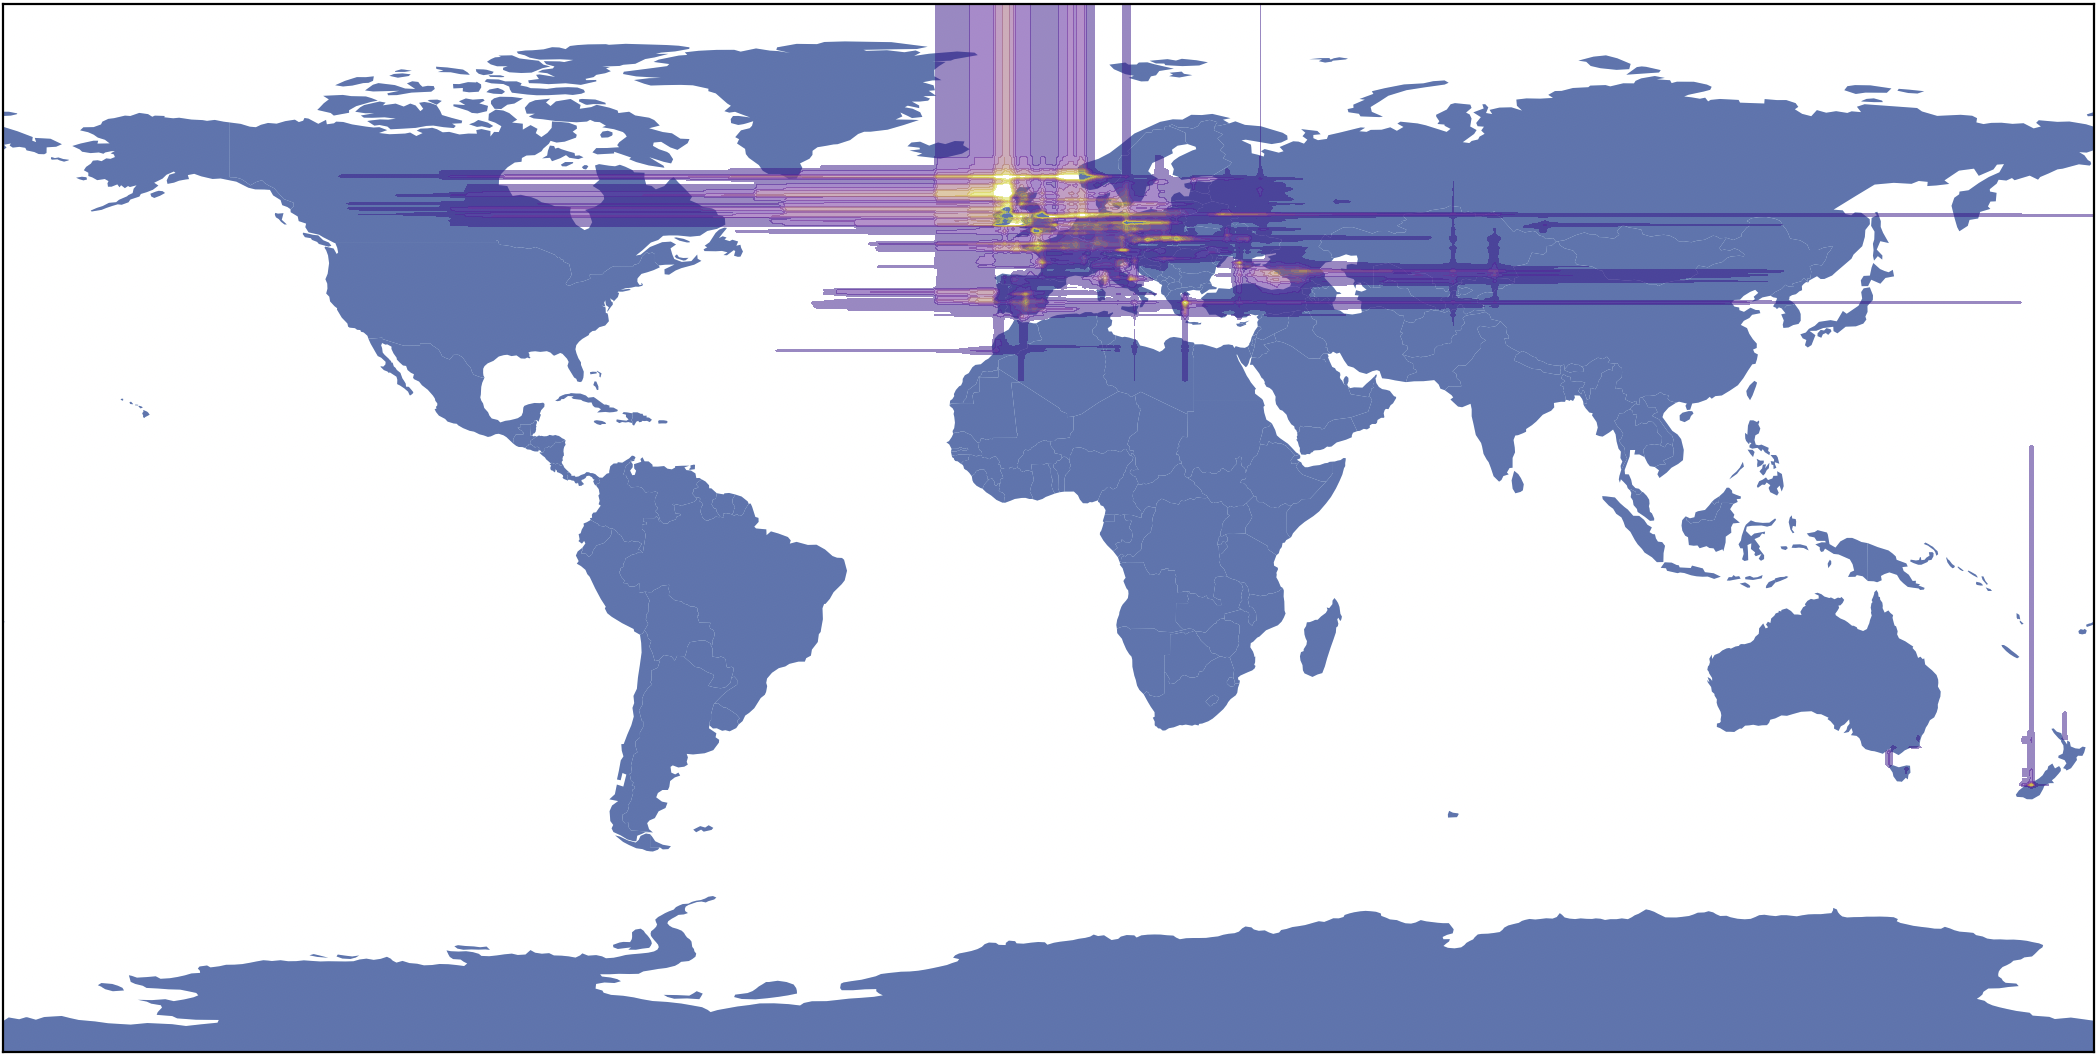
\includegraphics[width=\linewidth]{Images/RFcorrected.png} 
\vspace*{-3ex}  
\begin{center}
\textbf{Random Forest}
\end{center}
\end{subfigure} % <-- "\hfill"
\begin{subfigure}{.23\linewidth}
  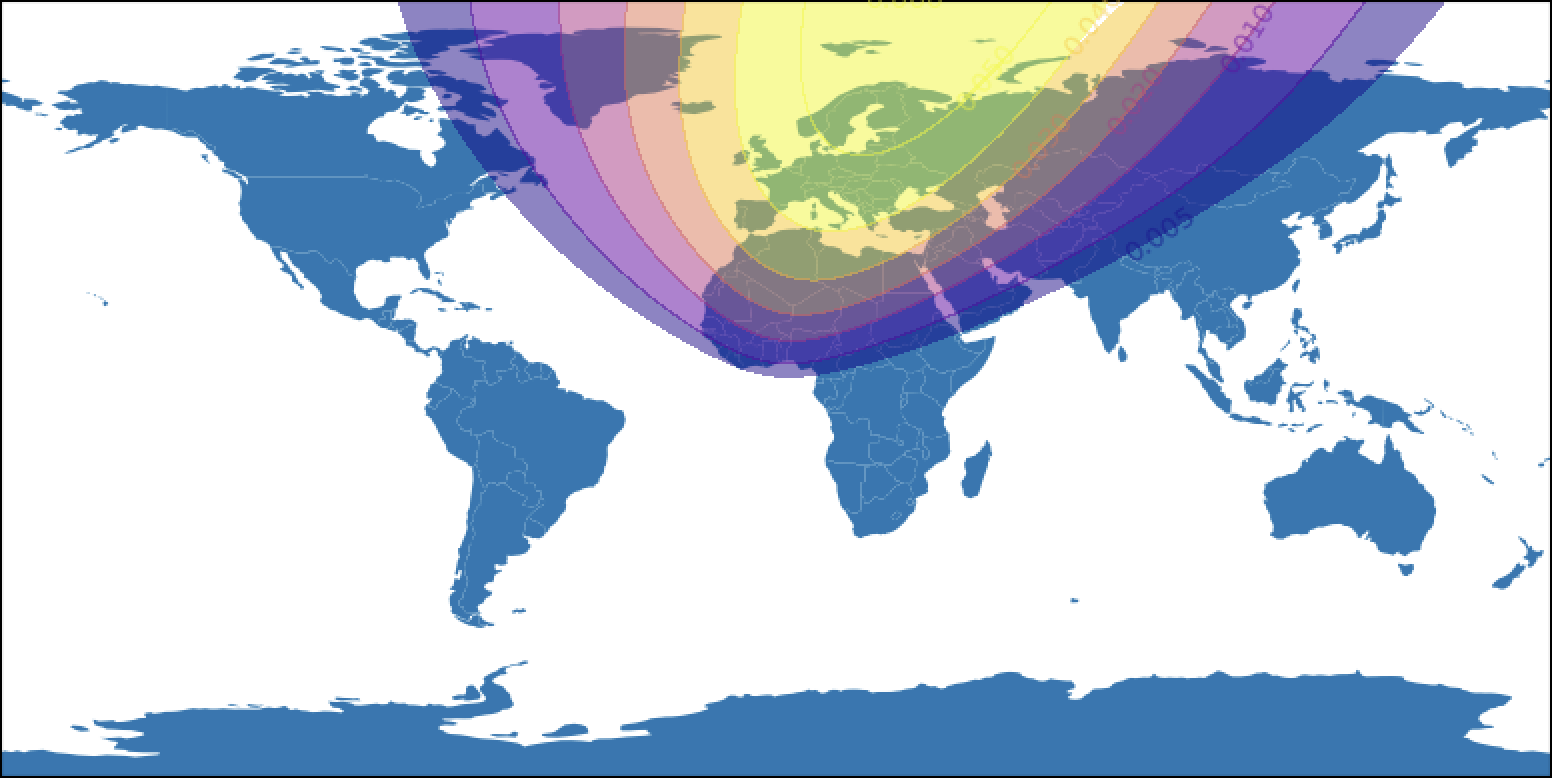
\includegraphics[width=\linewidth]{Images/Screenshot 2023-11-15 at 14.59.56.png}
\vspace*{-3ex}  
\begin{center}
\textbf{Logistic Regression}
\end{center}
\end{subfigure}
\begin{subfigure}{.04\linewidth}
  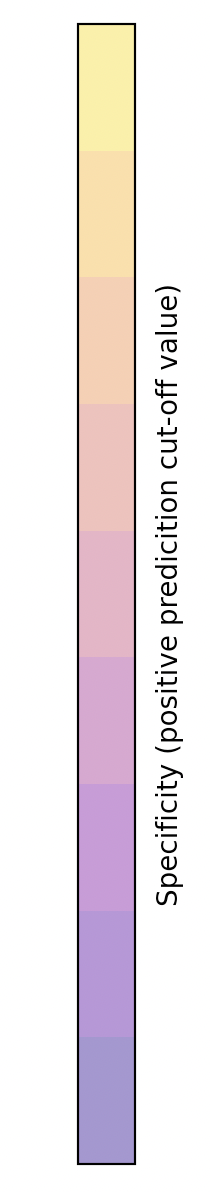
\includegraphics[width=\linewidth, height = 2.5cm]{Images/Screenshot 2023-11-19 at 12.10.01.png}
\end{subfigure}


\caption{Predicted Turdus Merula distributions using various trained models (bottom left-right) vs.\ true distribution (top). Note: The heat-plot nature of the maps is distribution predictions at different model parameters i.e. varying prediction `cut-off' values.}
\label{fig:map}
\end{figure}


%From figure \ref{fig:analysis}, we see that models tend to achieve better AUC-ROC values with data that has smaller distributions compared to larger distributions \hl{why - same reason as the AUC PR, FPs will be way way less likely than TNs hence a FPR close to 0 for classes with small number of locations, this also explains the difference in the axes, can exlain them together in the next paragraph}. A variation in AUC-ROC is not observed in comparing dense vs sparse populations.

%The AUC-PR values indicate the opposite, where larger values for AUC-PR are found in both largely distributed species and densely populated species, whereas small distributions and sparse distributions attain low scores. This is because of the inherent imbalance in the data, the smallest and sparsest distributions were attributed to species in the data-set which had very low counts for example, \emph{Gallotia stehlini} (35990) the species with the smallest distribution had only 2 data points. 

%As a result of the discrepancy between AUC-ROC and AUC-PR values, F-scores and Cohen's Kappa measures were also evaluated. \hl{Here we could mention that results were similar but the NN generally outperforms the other models, to justify its use for the following sections?}

\subsection{Conclusion}

% \hl{Investigating different models' responses to different types of population distribution in the data-set unveiled best AUC-ROC performance for smaller-sized population distributions, however, this was coupled with the worst found AUC-PR scores. The opposite was true for the largest-sized population distributions.- already mentioned?} 
Analyzing our models it is clear that some models are more adept at predicting different population distributions. RF and KNN performed better on average with small and sparse distributions, whereas FFNN performed better with larger distributions.
The Random Forest algorithm consistently did best averaged over all species (0.92, 0.18, 0.99, 0.37 for AUC-ROC, AUC-PR, CK, and F2-score respectively), importantly, however, all models returned very low AUC-PR values. To mitigate our models collective, consistently low AUC-PR results over all population distributions, we further investigate the addition of eight bio-climatic variables into the KNN, FFNN and RF algorithms and their response to the F2 metric.
% \footnote{\hl{The F2 metric specifically considered as we consider the importance of high precision and recall for the problem of SDM. - already mentioned?}}.


\section{Extended analysis of the effect of climate change on different species}

\subsection{Introduction of six new features}

Having been able to classify species at specific locations we now seek to implement new bio-climatic features to improve the prediction capabilities of our models. Annual temperature range, mean temperature of coldest quarter, mean temperature of warmest quarter, annual precipitation, precipitation of driest month, and precipitation seasonality data were sourced for all the locations in the train and test data-sets using WorldClim bio-climatic variables \cite{worldclim}, available at \url{https://www.worldclim.org/data/worldclim21.html}. Figures of these variables can be found in Appendix (\ref{appendix:bio}). Specifically, these new features allow models to produce more accurate results by isolating species predictions within ranges the species can tolerate, for example features like precipitation of driest month can help identify population distributions of desert-based species. The data sourced is restricted to land based, positive-only measurements. As a result, we reduce the task to only consider training for land based species, reducing the train data-set size to 271270. Future work could incorporate marine-based variables such as sea temperature, salinity, and ice content to build a more robust classifier capable of predicting the distribution of marine species in addition to terrestrial species. The Bio-ORACLE data-set \cite{oracle1} \cite{oracle2} would be suitable for this task. Each location data point within the training and test data-sets was combined with the six bio-climatic variables mentioned above, increasing the number of input features to eight. Upon training the models with the newly sourced features, an analysis of the models' F2 scores - specifically chosen due to sensitivity to precision and recall values - was evaluated, shown in Figure \ref{fig:8_feature}.

% \begin{figure}[htp]
% \centering
% \begin{tabular}{@{}c@{}}
% \subfloat{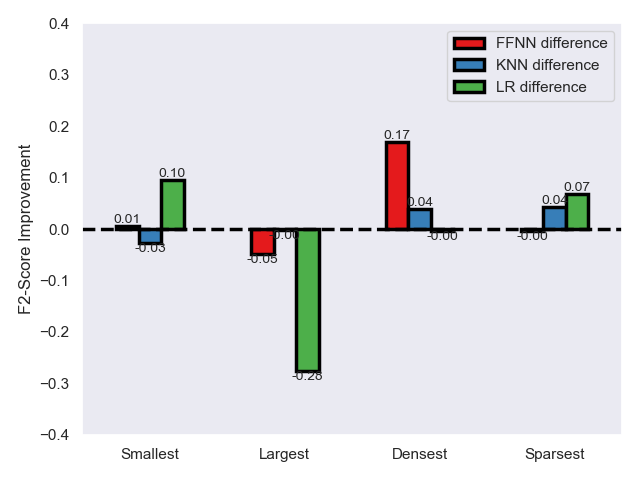
\includegraphics[width=0.4\linewidth]{Images/8_feature_improvement_preemptive.png}}\\
% \end{tabular} % some space
% \begin{tabular}{@{}c@{}}
% \subfloat{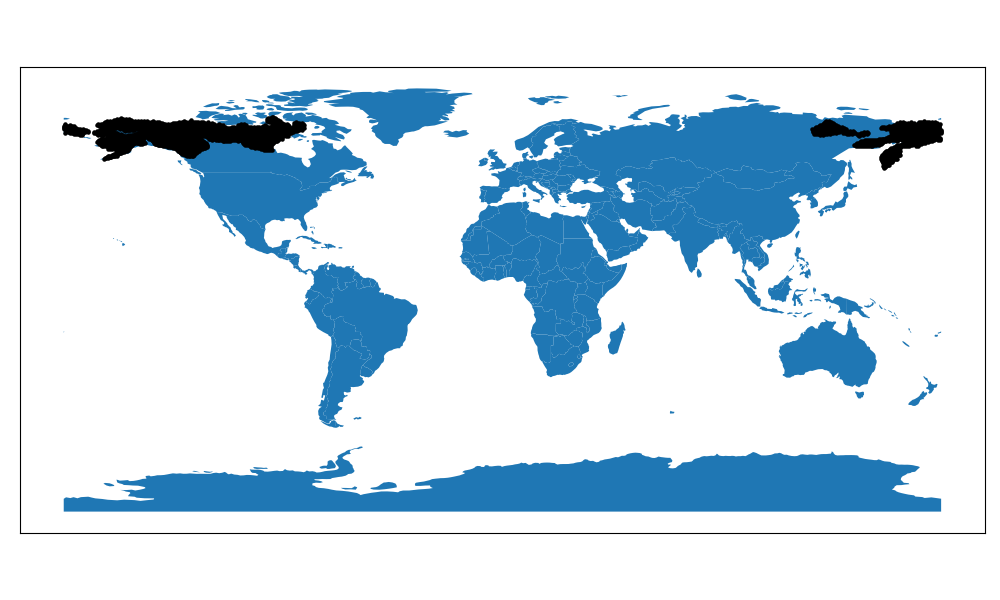
\includegraphics[width=0.25\linewidth]{Images/arctic squirrel true.png}}\\
% \subfloat{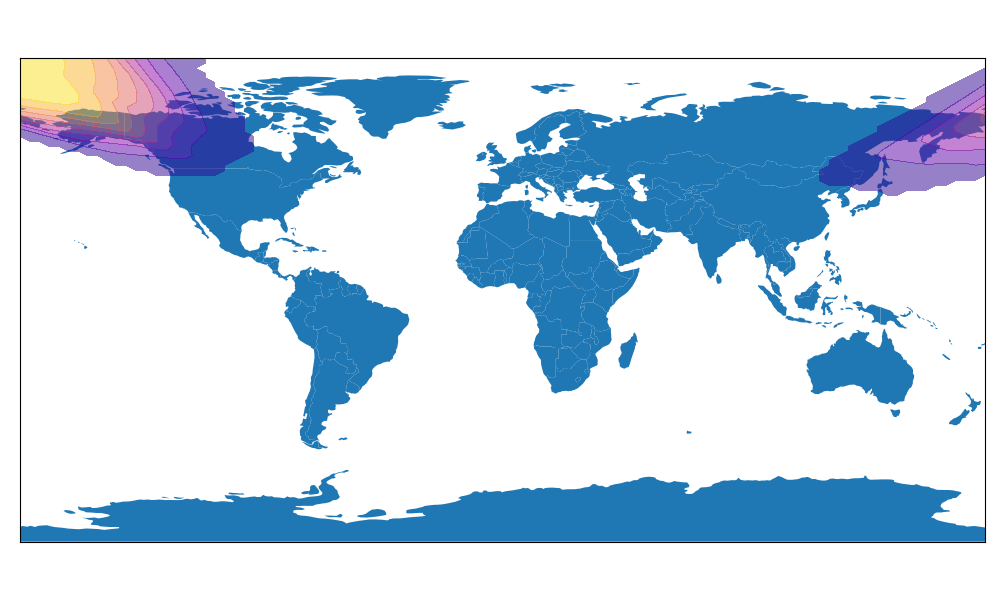
\includegraphics[width=0.25\linewidth]{Images/arctic squirrel 2 feature.png}}
% \subfloat{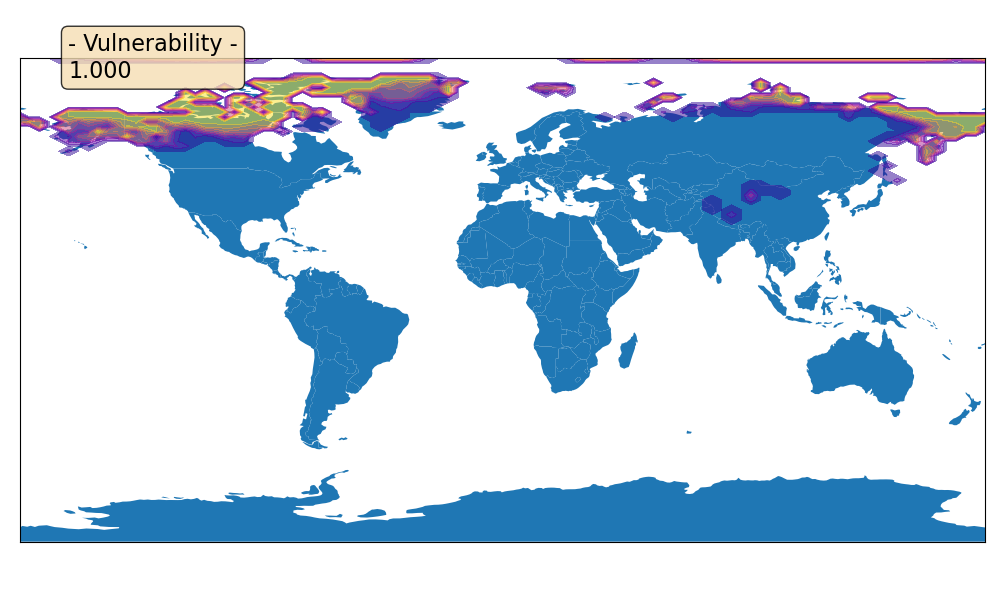
\includegraphics[width=0.25\linewidth]{Images/arctic squirrel vulnerability.png}}
% \\ 
% \end{tabular}
% \caption{Caption.}
% \end{figure}

\begin{figure}[hbt!]
\centering

\begin{subfigure}{.45\linewidth}
\vspace*{-1ex}  
\begin{center}
\textbf{F2 change; 2 feature vs 8 feature}
\end{center}
\vspace*{-1ex}
  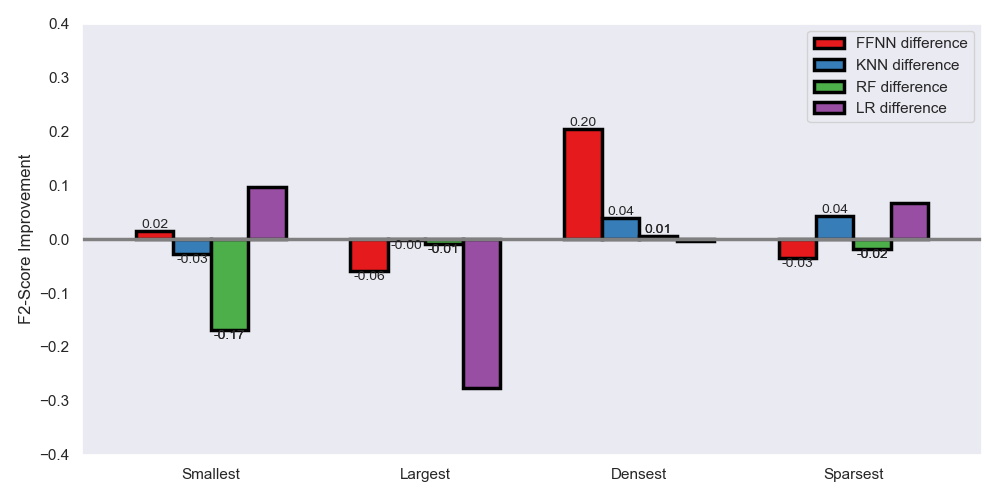
\includegraphics[width=\linewidth]{Images/F2 improvement.png}
\end{subfigure} \hspace{1em}  % <-- "\hfill"
\begin{subfigure}{.3\linewidth}
  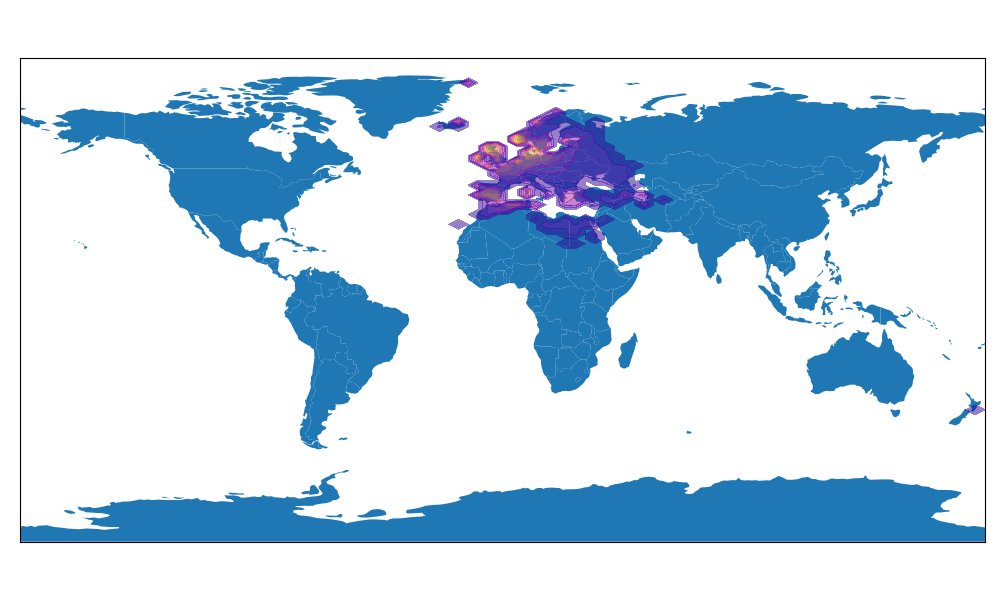
\includegraphics[width=\linewidth]{Images/8 feature turdus.png}
\vspace*{-5ex}  
\begin{center}
\textbf{FFNN-8 feature Turdus Merula}
\end{center}
\vspace{0ex}
\end{subfigure}
\begin{subfigure}{.04\linewidth}
  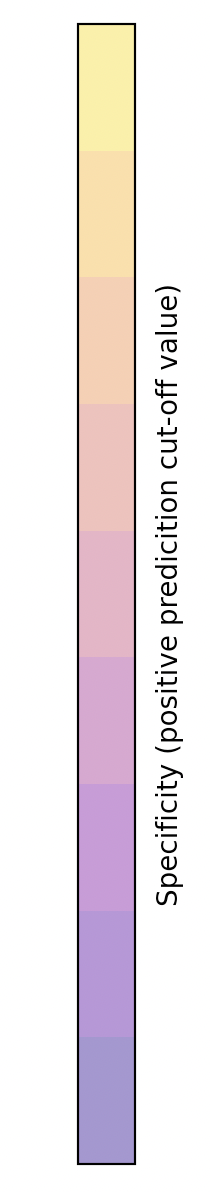
\includegraphics[width=\linewidth, height = 2.5cm]{Images/Screenshot 2023-11-19 at 12.10.01.png}
  \vspace{1ex}
\end{subfigure}

\caption{(Left) The metric improvements/losses when trained with new 8-feature data (land-based species only). (Right) Newly predicted Turdus Merula distribution from the FFNN (most improved).}
\label{fig:8_feature}
\end{figure}
As can be seen from Figure \ref{fig:8_feature}, the FFNN model experienced the biggest improvements. Notably, the models performed worse on some types of population distribution; this is because the new features help identify similar regions to that input, smaller distributed populations are then over-identified in a broader range of regions that would be `climatically suitable', as shown in appendix \ref{appendix:smalldistn}. Additionally, introducing 6 new features may have led to overfitting of the data, explaining the overall lower than expected improvement in F2 score.



% Figure \hl{X} shows the changes in accuracy of species distribution prediction with the introduction of the new features...

% A visual comparison of a predicted species distribution, \emph{Oenanthe leucopyga}, is shown in figure \ref{fig:extra_feature}

% \emph{Oenanthe Leucopyga} is known to inhabit desert, rocky areas; resident to the sahel regions in Africa, stretching into parts of the middle east \hl{cite}. The original models trained on 2-features fail to capture this behaviour, incorrectly predicting exact population distributions. The 8-feature trained models manage to capture population distributions by extending predictions beyond given limited location data into regions which would be suitable for species based on given location bioclimatic variables.


\subsection{Effect of climate change on newly trained models}
We now use a FFNN, combined with the new bio-climatic features, to predict species most at risk due to climate change. To quantify the effects of climate change, we examine the difference in yearly average temperatures between a baseline value, calculated as the mean over 30 years from 1984-2014, and a projected value for the year 2050, computed under the high emissions scenario (SSP5-8.5). The temperature data is taken from the Met Office Hadley Centre HadGEM3-GC31-LL model \cite{met}, prepared for the Coupled Model Intercomparison Project Phase 6 (CMIP6). A visualization of temperature anomaly is shown in appendix \ref{appendix:temp-anomaly}. Based on the 2050 temperature anomaly, we now compute a "score" that quantifies how extreme the predicted temperature increase of a particular location will be due to climate change, which is obtained by normalising the temperature anomaly by the largest increase (in this case 17$^\circ$C). We note that a few localised patches of ocean saw a decrease in yearly temperatures based on the model data, however, since these areas were small and the decrease was less than a degree, we set the temperature anomaly for these locations to 0$^\circ$C for the purposes of calculation. Combining this analysis of climate data at different locations with our models' improved prediction capability we can now provide accurate population distribution predictions and a `vulnerability' score for specific species as shown in Table \ref{tab:vulnerability}. We note that our vulnerability score is quite simplistic in the sense that a larger increase in temperature does not necessarily translate to a larger negative effect on a species, for example, certain species might be more resilient to changes in temperature than others. For future work, we might define this score differently by considering multiple climate metrics in addition to the yearly average temperature anomaly, for example, the anomalies in maximum temperature of the warmest month, lowest temperature of the coldest month, precipitation rates, sea ice content, etc. This would give a more complete evaluation of how climate change affects habitats beyond an increase in yearly average temperatures. Notably, species with high vulnerability were located near the poles (latitudes of $\approx 80$ and $\approx-80$ for the Arctic Ground Squirrel, shown in appendix \ref{appendix:arcticsq} and Chinstrap Penguin respectively), whereas species with low vulnerability were located in temperate regions between $\approx-50$ and $\approx-60$ latitude.


\begin{table}[hbt!]
\begin{tabular}{ |p{2cm}|p{2cm}|p{2cm}||p{2cm}|p{2cm}|p{2cm}|  }
 \hline
 \multicolumn{6}{|c|}{\textbf{Climate change vulnerability analysis}} \\
 \hline
 \rowcolor{lightgray} \footnotesize{\textbf{Most Vulnerable}}& \footnotesize{\textbf{Vulnerability}} & \footnotesize{\textbf{Location (largest pop.)}} & \footnotesize{\textbf{Least Vulnerable}} & \footnotesize{\textbf{Vulnerability}} & \footnotesize{\textbf{Location (largest pop.)}} \\
 \hline
\scriptsize{\emph{Arctic G. Squirrel}}  & \scriptsize{1.0 (298.15)} & \scriptsize{N.America} & \scriptsize{\emph{Black Rain Frog}} & \scriptsize{0.000002} & \scriptsize{Africa} \\
\scriptsize{\emph{Chinstrap Penguin}} & \scriptsize{0.70}  & \scriptsize{Antarctica} & \scriptsize{\emph{Whistling Tree Frog}} & \scriptsize{0.000012} & \scriptsize{Australia} \\
\scriptsize{\emph{Pine Grosbeak}} & \scriptsize{0.38} & \scriptsize{N.America} & \scriptsize{\emph{Golden C. Snake}} & \scriptsize{0.000012} & \scriptsize{Australia} \\
\scriptsize{\emph{Common Redpoll}} & \scriptsize{0.20} & \scriptsize{Europe}  & \scriptsize{\emph{Cape Mole Rat}} & \scriptsize{0.000015} & \scriptsize{Africa} \\
\scriptsize{\emph{Ruffed Grouse}} &  \scriptsize{0.18}  & \scriptsize{N.America} & \scriptsize{\emph{Tusked Frog}} & \scriptsize{0.000016} & \scriptsize{Australia} \\

 \hline
\end{tabular}
\caption{An analysis of the most and least vulnerable species to climate change. Scores were scaled according to that achieved by the most vulnerable species.}
\label{tab:vulnerability}
\end{table}
\vspace{-3ex}


\section{Conclusion}
We trained four different machine learning models on a data-set from iNaturalist containing coordinates and names of species identified at those coordinates. The four models used were a Feed-Forward Neural Network (FFNN), Random Forest (RF), Logistic Regression (LR), and K-Nearest Neighbours (KNN). We evaluated the performance of these models on the test-data by calculating the PRAUC, ROCAUC, F2-score, and Cohen's kappa for different subsets of species, as well as an all-species mean. From this, it was determined that the random forest performed the best under our chosen metrics.
%We trained four different machine learning models on a data-set from iNaturalist containing coordinates and names of species identified at those coordinates. The four models used were a feed-forward neural network, random forest, logistic regression, and k-nearest neighbours. We evaluated the performance of these models on a test set by calculating the precision-recall area-under-curve, receiver operating characteristic area-under-curve, F2 score, and Cohen's kappa for different subsets of species in the test set, as well as an all-species mean. From this, it was determined that the random forest performed the best under our chosen metrics.
To improve the accuracy of our models we introduced six bio-climatic features and trained the KNN, FFNN and RF models on these features in addition to the given geospatial data. Overall, this led to some increases in F2 score, particularly for dense populations in the FFNN model. Using past and projected future temperature values, we determined the species that are most likely to be affected by climate change. We defined a "vulnerability score" and in conjunction with the improved eight-feature FFNN, was used to determine that the species in Table \ref{tab:vulnerability} are the most likely to be affected by climate change.

%by normalising the temperature anomaly across the Earth by the largest difference. This score, in conjunction with the improved eight-feature FFNN, was used to determine that the species in table\ref{tab:vulnerability} are the most likely in the given data-set to be affected by climate change.


\newpage


\bibliography{refs.bib}
\bibliographystyle{unsrt}


\section*{Statement of Contribution}
\underline{s1910360}: Species distribution types (spans and densities), implementation and testing of FFNN (2-feature, 8-feature and vulnerability implementation), 8-feature data-set creation.

\underline{s2572047}: Background reading and write-up. Implementation and testing of KNN and LR. Obtaining temperature anomaly data.

\underline{s1922260}: Continent data exploration and data preparation. Implementation and testing of Random Forest. Overall analysis of results. 
 

\appendix
\section{Data structure summary of the train and test data-sets}\label{appendix:datastruct}

\begin{table}[H]
\begin{tabular}{ |p{3cm}||p{3cm}|p{3cm}|p{3cm}|  }
 \hline
 \multicolumn{4}{|c|}{\textbf{Data structure}} \\
 \hline
 \rowcolor{lightgray} \footnotesize{\textbf{Data-set}}& \footnotesize{\textbf{\#Data-points}} & \footnotesize{\textbf{\#Unique species}} & \footnotesize{\textbf{Mean \#locs per species}}\\
 \hline
 \footnotesize{\textbf{Train}}   & \footnotesize{272037}    & \footnotesize{500} &   \footnotesize{544}\\
 \footnotesize{\textbf{Test}} &   \footnotesize{288122}  & \footnotesize{500}   &\footnotesize{3413}\\

 \hline
\end{tabular}
\caption{Data structure of the provided data-sets `train' and `test'.}
\label{tab:my_label}
\end{table}



\section{Species observation count per. continent}\label{appendix:table1}

\begin{table}[H]
\begin{tabular}{ |p{3cm}||p{3cm}|p{3cm}|p{3cm}|  }
 \hline
 \rowcolor{lightgray} \footnotesize{\textbf{Continents}}& \footnotesize{\textbf{\#Observations}} & \footnotesize{\textbf{\#Species}} & \footnotesize{\textbf{Average \#Observations per Species}}\\
 \hline
 \footnotesize{\textbf{N. America}}   & \footnotesize{126579}    & \footnotesize{134} &   \footnotesize{944.6}\\
 \footnotesize{\textbf{Europe}}   & \footnotesize{34774}    & \footnotesize{34} &   \footnotesize{1022.8}\\
 \footnotesize{\textbf{Oceania}}   & \footnotesize{35763}    & \footnotesize{73} &   \footnotesize{489.9}\\
 \footnotesize{\textbf{Asia}}   & \footnotesize{22317}    & \footnotesize{67} &   \footnotesize{333.1}\\
 \footnotesize{\textbf{Africa}}   & \footnotesize{32737}    & \footnotesize{122} &   \footnotesize{268.3}\\
 \footnotesize{\textbf{S. America}}   & \footnotesize{19659}    & \footnotesize{69} &   \footnotesize{284.9}\\
 \footnotesize{\textbf{Antarctica}}   & \footnotesize{208}    & \footnotesize{1} &   \footnotesize{208}\\
 \hline
\end{tabular}
\caption{Number of Observations, Number of Species ann Average Number of Observations per Species for each Continent.}

\end{table}


\section{Feed-Forward Neural Network Architecture} \label{appendix:ffnn}
\begin{figure}[h]
\centering
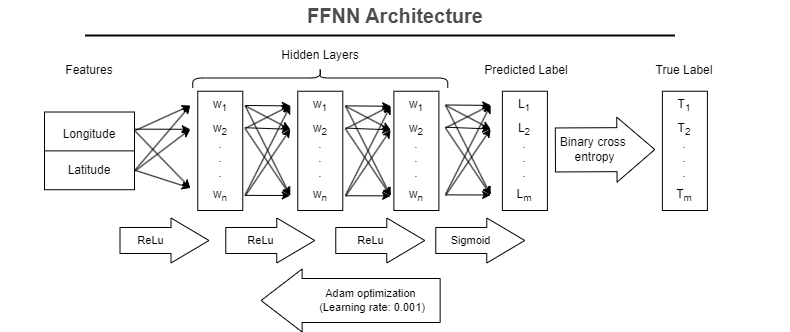
\includegraphics[width = .6\textwidth]{Images/neural_net.png}
\caption{Feed-forward neural network architecture used to predict species on location data.}
\label{FFNNarchitecture}
\end{figure}


\section{Random Forest Optimisation}\label{appendix:RFF1}

\begin{figure}[H]
\centering
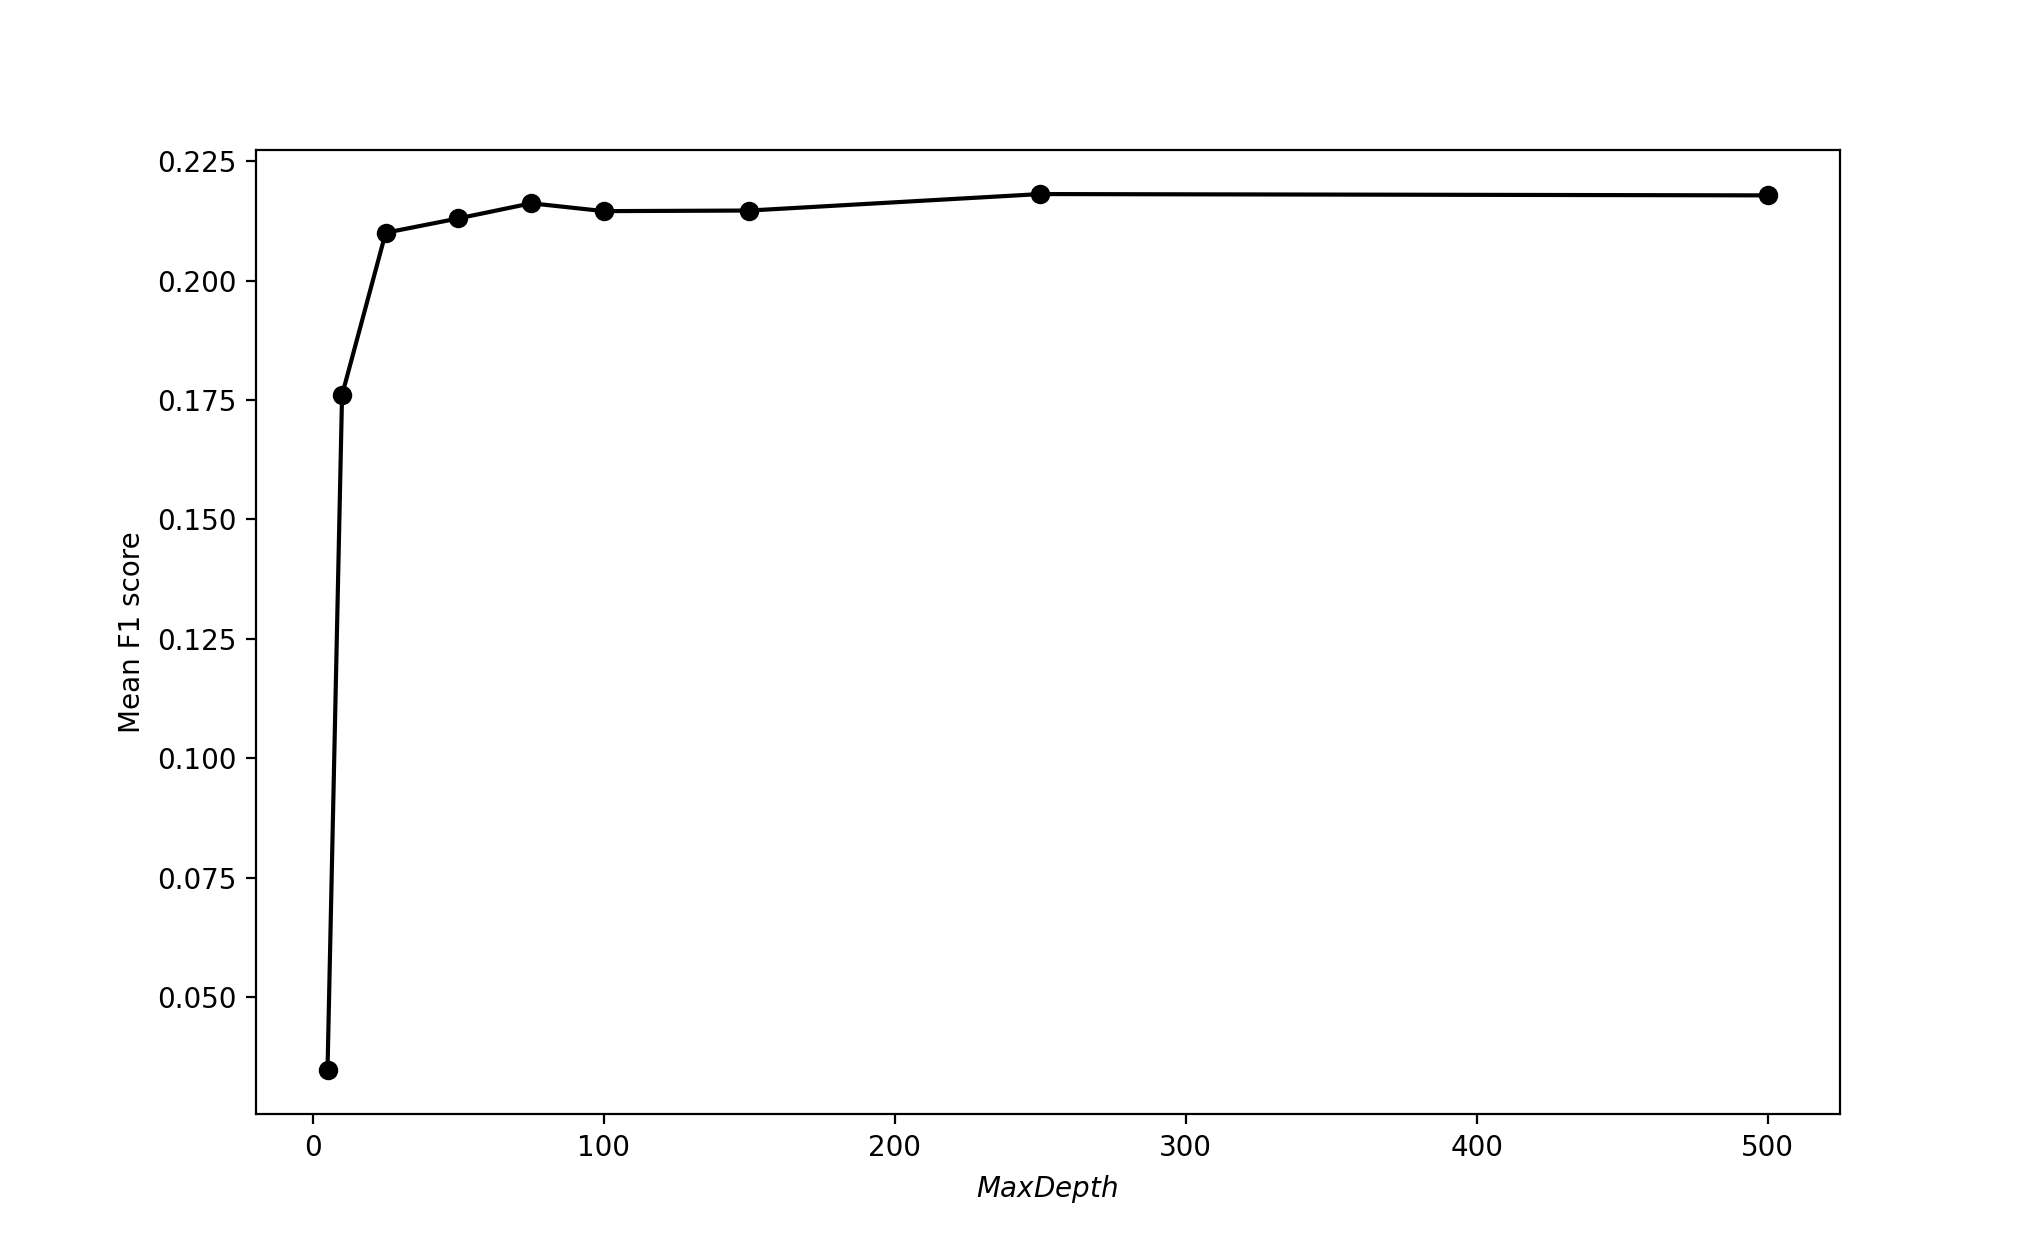
\includegraphics[width = .6\textwidth]{Images/Appendix.png}
\caption{Mean F1 score across all species for different values of maximum depth. At \textit{max\_depth=10} the F-score plateaus.}
\label{RFF1}
\end{figure}


\section{KNN Optimisation} \label{appendix:KNNF1}

\begin{figure}[H]
\centering
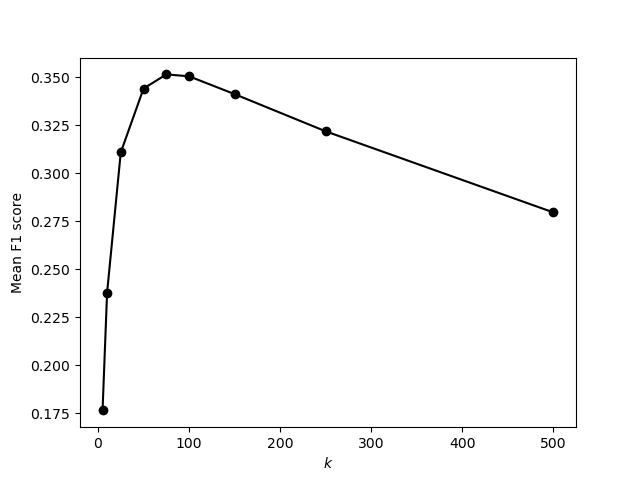
\includegraphics[width = .6\textwidth]{Images/knn_f1_scores.png}
\caption{Mean F1 score across all species for different values of k, the number of nearest neighbours used in KNN classification. The maximum value corresponds to $k = 75$.}
\label{KNNF1}
\end{figure}




\section{Bioclimatic variables} \label{appendix:bio}

\begin{figure}[H]
\label{appendix:extra}
\centering

\begin{subfigure}{.3\linewidth}
  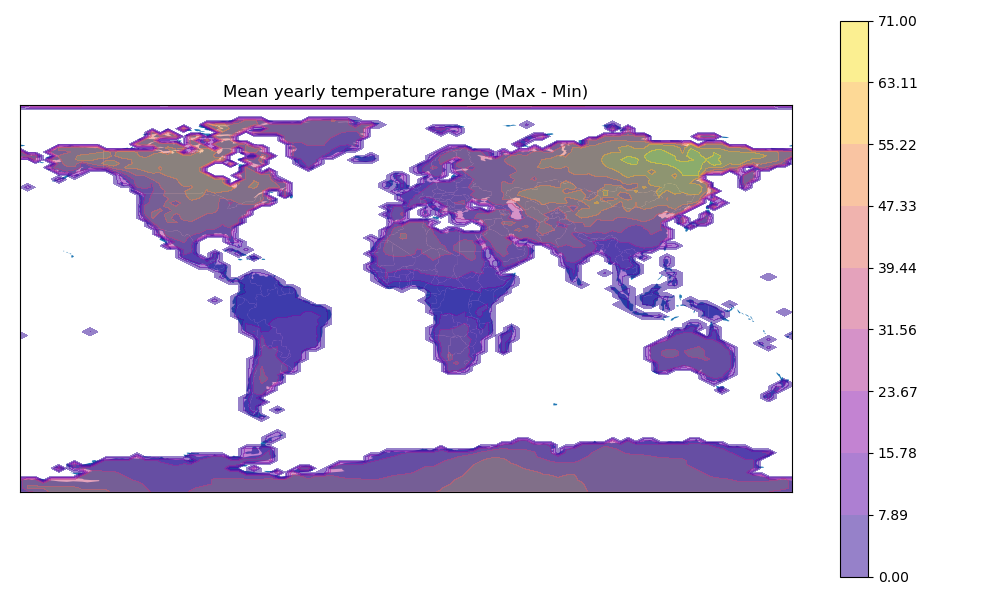
\includegraphics[width=\linewidth]{Images/mean_temp.png}

\end{subfigure}
\begin{subfigure}{.3\linewidth}
  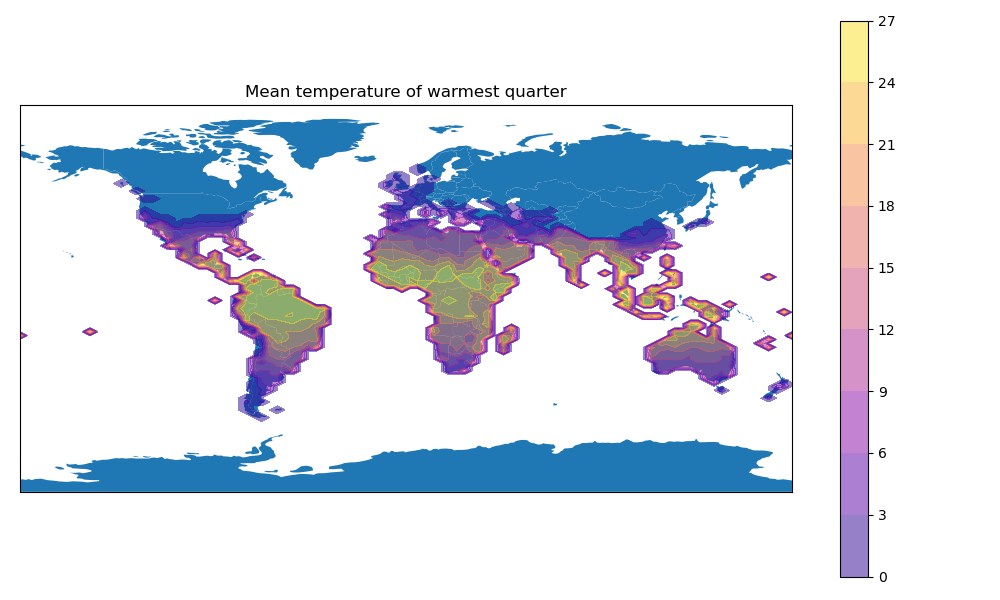
\includegraphics[width=\linewidth]{Images/mean_temp_warm.png}

\end{subfigure}
\begin{subfigure}{.3\linewidth}
  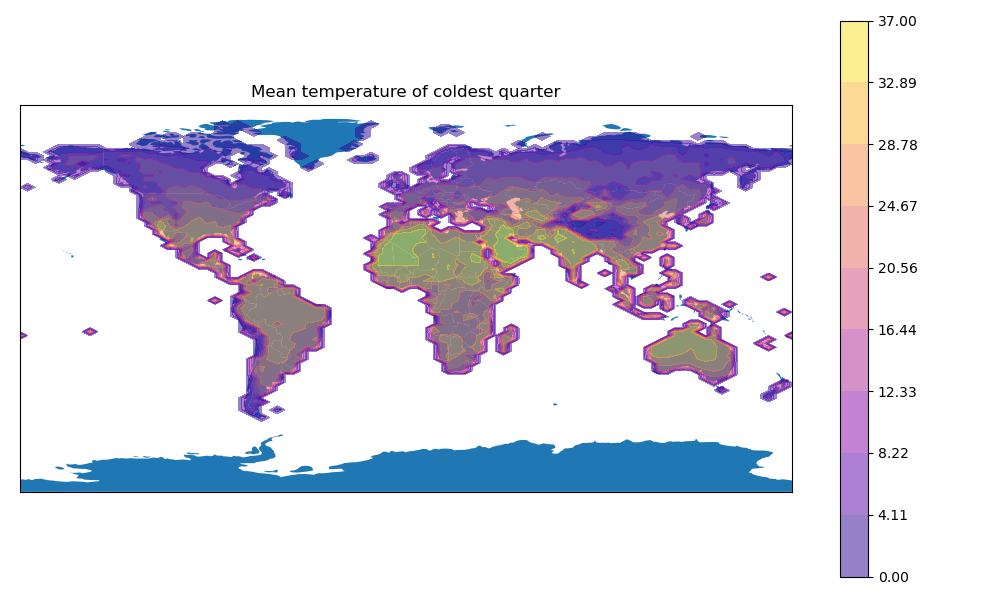
\includegraphics[width=\linewidth]{Images/mean_temp_cold.png} 

\end{subfigure} 

\begin{subfigure}{.3\linewidth}
  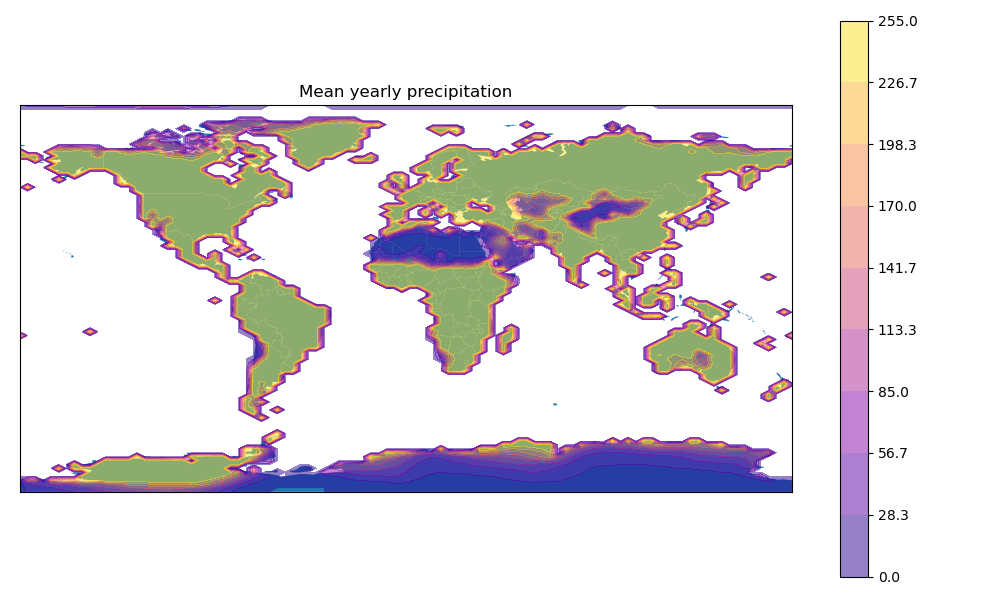
\includegraphics[width=\linewidth]{Images/mean_precip.png}

\end{subfigure}
\begin{subfigure}{.3\linewidth}
  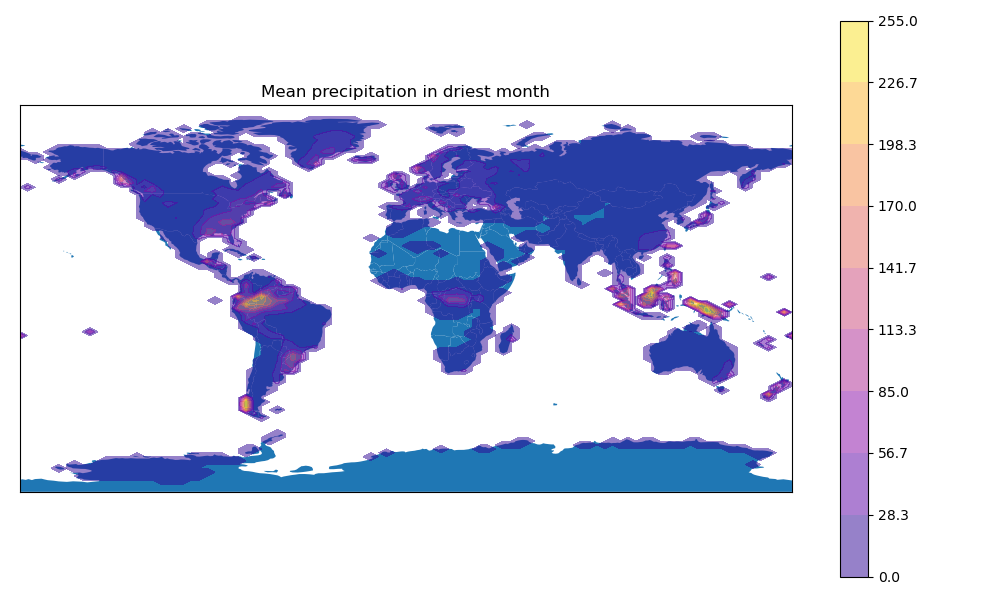
\includegraphics[width=\linewidth]{Images/mean_precip_dry.png}

\end{subfigure}
\begin{subfigure}{.3\linewidth}
  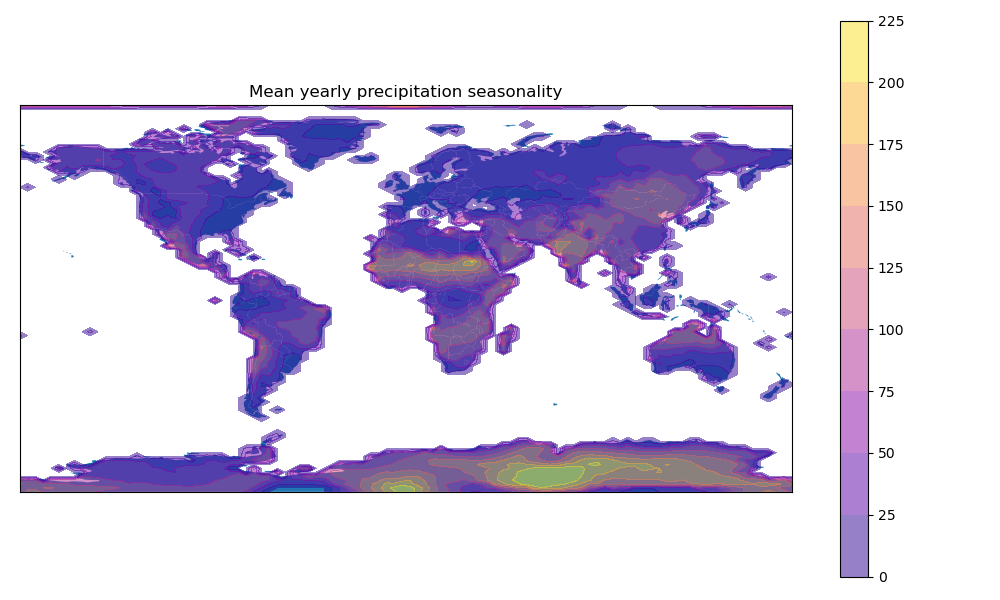
\includegraphics[width=\linewidth]{Images/mean_precip_seasonality.png} 

\end{subfigure} 

\caption{Bio-climatic variables introduced to further train models. (Top) from right to left is the mean yearly temperature range, mean temperature of the warmest quarter, and mean temperature of the coldest quarter.
(Bottom) from right to left is the mean yearly precipitation, mean precipitation in the driest month, and mean precipitation seasonality.}
\label{fig:extra}
\end{figure}

\section{Over estimation of small-distribution species with 8-feature model}\label{appendix:smalldistn}

\begin{figure}[H]
\centering

\begin{subfigure}{.4\linewidth}
  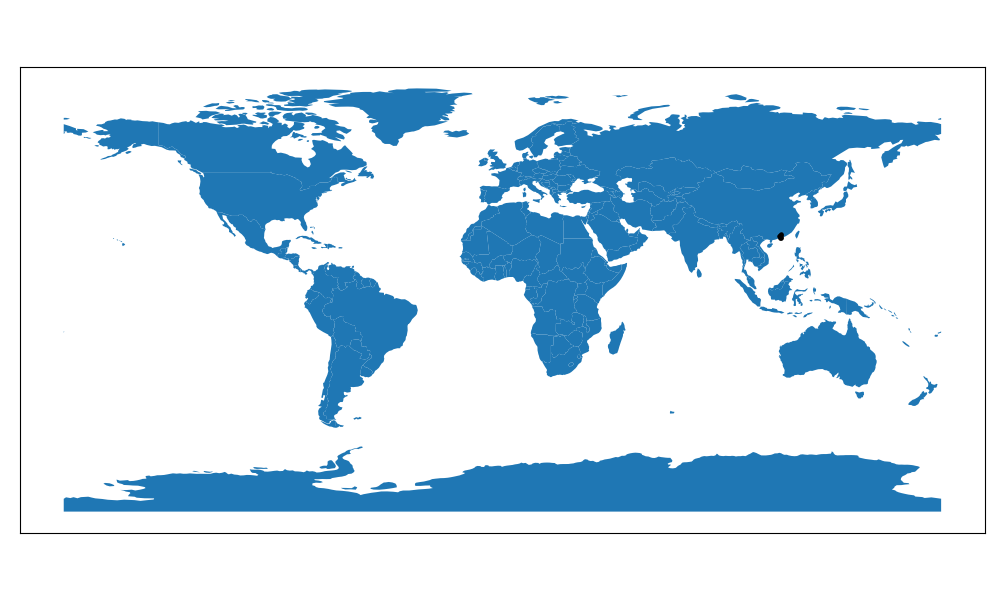
\includegraphics[width=\linewidth]{Images/small_distn_true.png}

\end{subfigure}
\begin{subfigure}{.4\linewidth}
  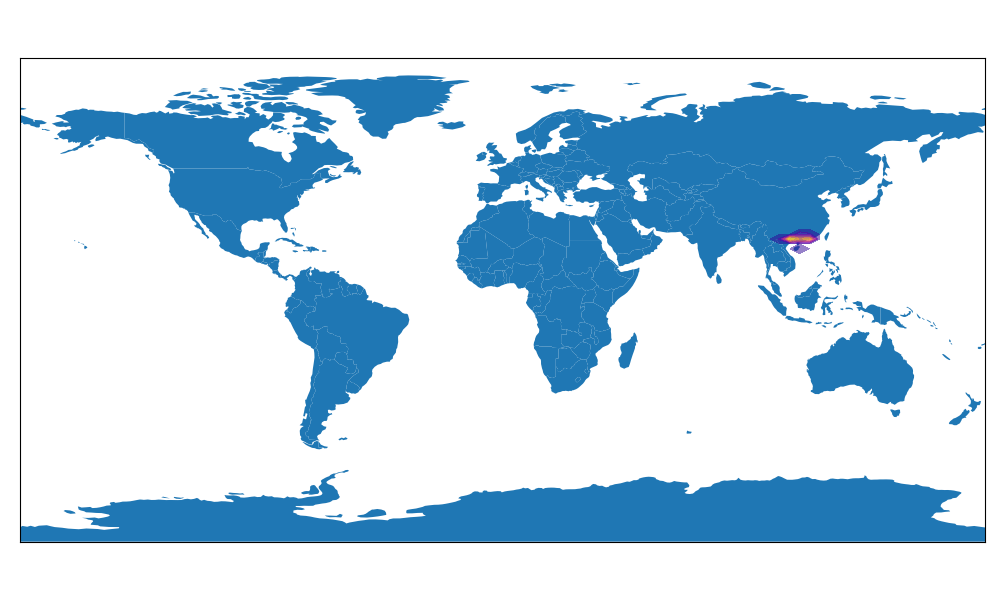
\includegraphics[width=\linewidth]{Images/small_distn_overestimation.png}

\end{subfigure}
\caption{Overestimation of species from the small-population distribution sample (taxon ID 64387) with the use of FFNN trained with bio-climatic variables.}
\end{figure}

\section{Temperature anomaly} \label{appendix:temp-anomaly}

\begin{figure} [H]
    \centering
    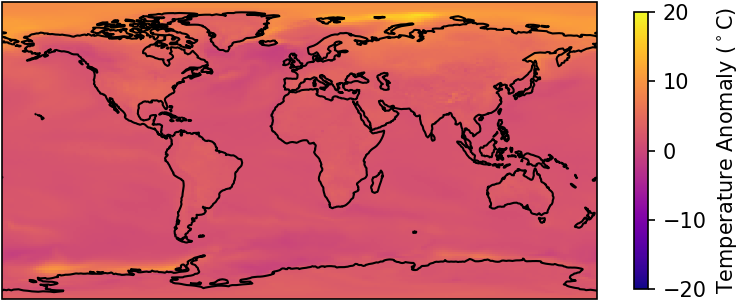
\includegraphics[width=0.5\linewidth]{Images/temp_anomaly.png}
    \caption{Projected yearly average temperature anomaly for 2050 compared to 1984-2014 baseline}
\end{figure}



\section{Arctic Ground Squirrel predicted distribution 8-feature FFNN} \label{appendix:arcticsq}

\begin{figure} [H]
    \centering
\vspace*{-1ex}  
\begin{center}
\textbf{Arctic G. Squirrel predicted distribution + vulnerability}
\end{center}
\vspace*{0ex}
    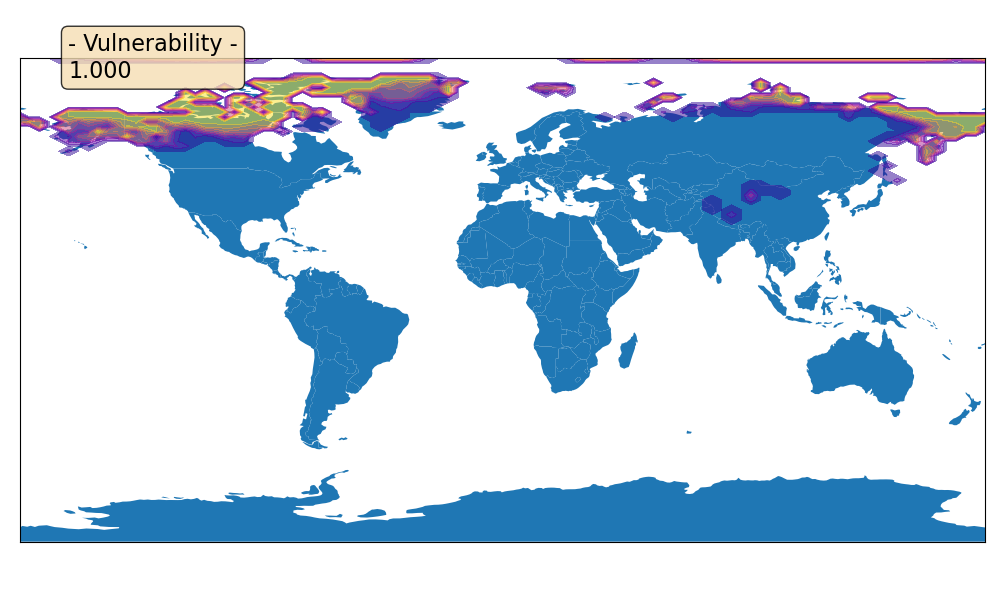
\includegraphics[width=0.5\linewidth]{Images/arctic squirrel vulnerability.png}
    \caption{8-feature FFNN population distribution prediction for the most vulnerable species in the data-set (\emph{Arctic Ground Squirrel}) alongside its scaled vulnerability score, 1.0, indicating the highest net-affect as a result of temperature anomaly.}
    \label{fig:arcticsq}
\end{figure}


\end{document}

%%% Local Variables:
%%% mode: latex
%%% TeX-master: t
%%% End:
